\documentclass[%
  a4paper,fontsize=11pt,abstract=on,%
  oneside,BCOR=19mm,% for print version adapt...
  %final % activate for final submission, removes draft status and date
]{scrreprt}
\defaulthyphenchar=127  % make all hyphens additional

% encoding (keep this and use UTF-8)
\usepackage[utf8]{inputenc}
\usepackage[T1]{fontenc}

% select the thesis language
% \usepackage[ngerman]{babel}  % select this for a German thesis
\usepackage[english]{babel}  % select this for an English thesis


% file with common and simple user defs

% set these accordingly
\newcommand{\myThesisType}{Bachelor / Master Thesis}  % Master Thesis / Seminararbeit
\newcommand{\myName}{Your Name}
\newcommand{\myLocation}{Your City}
\newcommand{\myTitle}{Title of this work}
\newcommand{\mySubtitle}{Subtitle / Subject}
\newcommand{\myKeywords}{Keywords describing this work}
\newcommand{\myThesisStudyCourse}{Computer Science}
\newcommand{\myThesisStudyCourseGerman}{Informatik}
\newcommand{\myThesisSupervisorExternal}{Dr.\ Someone External}
\newcommand{\myThesisExternalCompany}{Some Company}
\newcommand{\myProf}{Prof.\ Dr.\ Someone}
\newcommand{\myOtherProf}{Prof.\ Dr.\ SomeoneElse}
\newcommand{\myThesisSubDate}{2024-07-26}  % Put your submission date here, the Draft date will disappear when you set the "final" documentclass option in the thesis.tex


% you can define simple other commands here...
% if you want to do something more fancy or import other packages
% you probably want to just modify FrontBackmatter/preabmle.tex


% file taking care of imports, setup etc.
% some basic setting and imports
\usepackage{etoolbox} % extended toolbox for macros
\usepackage{xspace} % to get the spacing after macros right

\usepackage{csquotes} % dealing with "quotes" easily/properly
\MakeOuterQuote{"}

\usepackage[iso,\languagename]{isodate} % e.g., 2023-02-28
\usepackage{datetime2}
\usepackage{iflang} % \IfLanguageName{ngerman}{Deutsche Version}{English Version}

% get us an \IfFinal{in case final}{in case not final} command
\makeatletter\@ifclasswith{scrreprt}{final}{
    \newcommand{\IfFinal}[2]{#1}
}{
    \newcommand{\IfFinal}[2]{#2}
}\makeatother

% in case something uses these
\title{\myTitle}
\author{\myName}
\date{\IfFinal{\myThesisSubDate}{\today}}



% basic packages
%\usepackage{geometry} % clashes with BCOR
\usepackage[dvipsnames]{xcolor}
\usepackage{graphicx}
\usepackage{svg}
\usepackage{tikz}
\usetikzlibrary{calc}

% floats: tables, (sub)figures, and captions
\usepackage{tabularx} % better tables
  \setlength{\extrarowheight}{2pt} % increase table row height
\newcommand{\tableheadline}[1]{\multicolumn{1}{c}{\spacedlowsmallcaps{#1}}}
\newcommand{\myfloatalign}{\centering} % to be used with each float for alignment
\usepackage{caption}
\usepackage{makecell}
\usepackage{multirow} % Required to enable merging of columns/rows in a table
\usepackage{longtable}
\captionsetup{font=small} % format=hang,
\usepackage{subfig}
%\usepackage{varwidth}  % like minipage but "up to width"
%\usepackage{afterpage}
%\usepackage[below]{placeins}
\usepackage{rotating} % Required to display sideways tables/figures

% math packages
% \PassOptionsToPackage{fleqn}{amsmath}  % math environments and more by the AMS
\usepackage{amsmath}
\usepackage{amsfonts}
\usepackage{amssymb}
%\usepackage{amsthm}
%\usepackage{marginnote}
%\usepackage{mathtools}
%\usepackage{complexity}
%\usepackage{siunitx}
%\usepackage{bm} % Required for showing math symbols in boldface


% math formulae:
\renewcommand{\vec}[1]{\mathbf{#1}}
\newcommand{\lO}{\mathcal{O}}
\DeclareMathOperator*{\avg}{avg}



\usepackage{hyperref}
\definecolor{webgreen}{rgb}{0,.5,0}  % as in classicthesis
\definecolor{webbrown}{rgb}{.6,0,0}
\hypersetup{
  % draft, % hyperref's draft mode, for printing see below
  % uncomment the following line if you want to have black links (e.g., for printing)
  %colorlinks=false, linktocpage=false, pdfstartpage=1, pdfstartview=FitV, pdfborder={0 0 0},%
  %urlcolor=Black, linkcolor=Black, citecolor=Black, %pagecolor=Black,%
  colorlinks=true, linktocpage=true, pdfstartpage=1, pdfstartview=FitV,%
  urlcolor=webbrown, linkcolor=RoyalBlue, citecolor=webgreen, %pagecolor=RoyalBlue,%
  breaklinks=true, pdfpagemode=UseNone, pageanchor=true, pdfpagemode=UseOutlines,%
  plainpages=false, bookmarksnumbered, bookmarksopen=true, bookmarksopenlevel=1,%
  hypertexnames=true, pdfhighlight=/O,%nesting=true,%frenchlinks,%
  pdftitle={\myTitle},
  pdfsubject={\mySubtitle},
  pdfauthor={\myName},
  pdfcreator={pdfLaTeX},
  pdfkeywords={\myKeywords}
}


% good for \autoref{}
\addto\extrasenglish{% only works with \usepackage[english]{babel}
  \renewcommand*{\partautorefname}{Part}%
  \renewcommand*{\chapterautorefname}{Chapter}%
  \renewcommand*{\sectionautorefname}{Section}%
  \renewcommand*{\subsectionautorefname}{Section}%
  \renewcommand*{\subsubsectionautorefname}{Section}%
  \renewcommand*{\paragraphautorefname}{Paragraph}%
  \renewcommand*{\subparagraphautorefname}{Paragraph}%
  \renewcommand*{\appendixautorefname}{Appendix}%
  \renewcommand*{\pageautorefname}{Page}%
  \renewcommand*{\figureautorefname}{Figure}%
  \renewcommand*{\tableautorefname}{Table}%
  \renewcommand*{\footnoteautorefname}{Footnote}%
  \renewcommand*{\FancyVerbLineautorefname}{Line}%
  \renewcommand*{\theoremautorefname}{Theorem}%
  \renewcommand*{\equationautorefname}{Equation}%
  \renewcommand*{\itemautorefname}{Item}%
}%
\addto\extrasngerman{%
  \renewcommand*{\partautorefname}{Teil}%
  \renewcommand*{\chapterautorefname}{Kapitel}%
  \renewcommand*{\sectionautorefname}{Abschnitt}%
  \renewcommand*{\subsectionautorefname}{Abschnitt}%
  \renewcommand*{\subsubsectionautorefname}{Abschnitt}%
  \renewcommand*{\paragraphautorefname}{Absatz}%
  \renewcommand*{\subparagraphautorefname}{Absatz}%
  \renewcommand*{\appendixautorefname}{Anhang}%
  \renewcommand*{\pageautorefname}{Seite}%
  \renewcommand*{\figureautorefname}{Abbildung}%
  \renewcommand*{\tableautorefname}{Tabelle}%
  \renewcommand*{\footnoteautorefname}{Fußnote}%
  \renewcommand*{\FancyVerbLineautorefname}{Zeile}%
  \renewcommand*{\theoremautorefname}{Theorem}%
  \renewcommand*{\equationautorefname}{Gleichung}%
  \renewcommand*{\itemautorefname}{Punkt}%
}%
\providecommand{\subfigureautorefname}{\figureautorefname}





% ***************
% biblatex setup
% ***************
\PassOptionsToPackage{%
  backend=biber,%bibencoding=utf8, %instead of bibtex
  safeinputenc=true,
  %backend=bibtex8,bibencoding=ascii,%
  language=auto,%
  style=numeric-comp,%
  %style=authoryear-comp, % Author 1999, 2010
  %style=iso-authoryear,%
  %bibstyle=authoryear,dashed=false, % dashed: substitute rep. author with ---
  giveninits=true, % abbreviate firstnames
  sorting=nyt, % name, year, title
  maxbibnames=10, % default: 3, et al.
  backref=true,%
  %isbn=false,
  natbib=true % natbib compatibility mode (\citep and \citet still work)
}{biblatex}
    \usepackage{biblatex}

% enable linebreaks in bib urls
\setcounter{biburlnumpenalty}{7000}
\setcounter{biburlucpenalty}{7000}
\setcounter{biburllcpenalty}{8000}

% add actual bibtex file
\addbibresource{literature.bib}

% KOMA settings for bib
\KOMAoptions{bibliography=totoc} % totocnumbered}
\KOMAoptions{listof=totoc}



% Setup for code listings
% \usepackage{listings}
% \usepackage{scrhack}  % useful workarounds for some package (e.g., listings) incompat with newer koma
% %\lstset{emph={trueIndex,root},emphstyle=\color{BlueViolet}}%\underbar} % for special keywords
% \lstset{%
%     language=Python,%[LaTeX]Tex,%C++,
%     morekeywords={PassOptionsToPackage,selectlanguage},
%     keywordstyle=\color{RoyalBlue},%\bfseries,
%     basicstyle=\small\ttfamily,
%     %identifierstyle=\color{NavyBlue},
%     commentstyle=\color{Green}\ttfamily,
%     stringstyle=\rmfamily,
%     numbers=none,%left,%
%     numberstyle=\scriptsize,%\tiny
%     stepnumber=5,
%     numbersep=8pt,
%     showstringspaces=false,
%     breaklines=true,
%     % frameround=ftff,
%     frame=single,
%     belowcaptionskip=.75\baselineskip
%     %frame=L
% }
%\usepackage{minted}  % listings alternative
%\usepackage{alltt}  % maybe also useful




% Layout stuff
% (recommendation: leave as is, unless forced by your supervisors)

% line spacing
% \usepackage[singlespacing]{setspace}

%% Fontsizes
% \RedeclareSectionCommand[
%     afterskip=0pt,
%     beforeskip=0pt
% ]{chapter}
% \setkomafont{chapter}{\large}
% \RedeclareSectionCommand[
%     afterskip=0pt,
%     beforeskip=4pt,
%     runin=false,
% ]{section}
% \setkomafont{section}{\normalsize}
% \RedeclareSectionCommand[
%     afterskip=0pt,
%     beforeskip=3pt,
%     runin=false
% ]{subsection}
% \setkomafont{subsection}{\normalsize}
% \setkomafont{subsubsection}{\normalsize}
% \setkomafont{caption}{\small}

%% Paragraph
% \KOMAoptions{parskip=half}


% Header & Footer
\usepackage[headsepline, automark]{scrlayer-scrpage} % plainheadsepline
\pagestyle{scrheadings}
% \clearpairofpagestyles
\addtokomafont{pagehead}{\small\normalfont}
% \ihead*{\myTitle}
% \ofoot*{\pagemark}



% other useful packages:
% \usepackage{pgfgantt}

% To-dos
% \usepackage{snaptodo}
% \usepackage[disable]{todonotes}  % disable % to just get rid of todonotes (for review)
\usepackage[obeyFinal]{todonotes}  % doc final will also disable remaining todonotes
%\usepackage{changebar}
\usepackage{verbatim}
\usepackage{lipsum}

\pdfminorversion=6



\begin{document}
\pagenumbering{roman}
\begin{titlepage}
    \thispagestyle{empty}

    % BG Logo (according to H-BRS corporate design guide)
    \begin{tikzpicture}[remember picture, overlay]
        \filldraw[color=black!5]($(current page.north west) + (0,-12)$) circle (\paperwidth * 5 / 14);
        \filldraw[color=white]($(current page.north west) + (0,-12)$) circle (\paperwidth * 3 / 14);
        \filldraw[color=black!5]($(current page.north east) + (0,-12)$) circle (\paperwidth * 5 / 14);
    \end{tikzpicture}

    \vspace{-2cm}
    {
    
\includegraphics[width=9.2cm]{FrontBackmatter/H-BRS-Logo mit Fachbereich Informatik_DE_EN.pdf}
    % 
\includegraphics{FrontBackmatter/H-BRS_Logo_A4.pdf}

    % \vspace{1em}
    % \noindent
    % \hspace{3.614cm}
    % \parbox{10cm}{
    % \sffamily
    % \large
    % \textbf{Fachbereich Informatik}\\
    % Department of Computer Science
    % }
    }

    \vfill
    \begin{center}

        \Large\normalfont\myThesisType\\[1ex]
        \large\normalfont\IfLanguageName{ngerman}{\myThesisStudyCourseGerman}{\myThesisStudyCourse}
        
        \vfill
        
        \Huge\normalfont\myTitle\\[1ex]
        \ifdefempty{\mySubtitle}{}{\huge\normalfont\mySubtitle}

        \vfill

        \Large\myName
        

        \vfill
        \vfill

        \large
        \begin{tabular}{ll}
            \ifdefempty{\myThesisSupervisorExternal}{}{%
                \IfLanguageName{ngerman}{Betreuer}{Supervisor}
                    & \myThesisSupervisorExternal \\}
            \ifdefempty{\myThesisExternalCompany}{}{%
                    & \myThesisExternalCompany    \\[1ex]}
            \IfLanguageName{ngerman}{Erstprüfer}{Examiner 1}
                & \myProf    \\
            \IfLanguageName{ngerman}{Zweitprüfer}{Examiner 2}
                & \myOtherProf   \\[2em]
            \IfFinal{}{\IfLanguageName{ngerman}{Vorabversion vom}{Draft as of} & \DTMnow\\
            & \small \IfLanguageName{ngerman}{(Zur Abgabe: \texttt{final} Option in thesis.tex setzen!)}{(For submission: set \texttt{final} option in thesis.tex!)}\\}
            \IfFinal{\IfLanguageName{ngerman}{Eingereicht am}{Submitted on} }{\IfLanguageName{ngerman}{Einzureichen am}{To be submitted on}}
                & \myThesisSubDate
        \end{tabular}
    \end{center}
\end{titlepage}


\begin{abstract}
This project report is part of the Search Query Writer (SQW) initiative by Fraunhofer INT, designed to assist researchers in generating comprehensive literature search queries, particularly in unfamiliar topic areas. A critical limitation in current literature search workflows is the absence of an objective evaluation framework for query performance, which has so far relied on subjective assessments. This study addresses this gap by introducing a curated dataset containing core publications, which are relevant publications identified through systematic literature reviews (SLRs) or bibliometric analysis works, across multiple research fields, alongside novel metrics to evaluate the query results. Recall and precision are traditionally used for literature search query evaluation, with recall being the primary metric to ensure the retrieval of relevant publications. However, literature searches often yield excessively large result sets, complicating the identification of core publications. To address this, we introduce \textit{semantic precision}, a metric that uses embedding space to identify possible true positives based on their semantic similarity to core publications. Our evaluation reveals that while SQW-generated queries outperform the baseline in recall, they often suffer in precision, particularly when query expansion introduces irrelevant keywords. Primarily, the main goal of this framework is to provide a systematic and automated approach to assess literature search queries. It lays the groundwork for improving tools like SQW, enabling more effective literature query generation across diverse research domains.

\end{abstract}



\cleardoublepage
\tableofcontents
% if your professor wants them...
 \listoffigures
% \listoftables

\cleardoublepage
\setcounter{page}{1}
\pagenumbering{arabic}


\chapter{Introduction}\label{ch:intro}

The Fraunhofer Institute for Technological Trend Analysis (INT)\footnote{\url{https://www.int.fraunhofer.de/}} specializes in conducting technology foresight, tackling tasks and research questions across a diverse array of fields. These challenges often necessitate systematic and scientifically sound approaches, even when prior knowledge in the domain is sparse. To address this recurring need, a tool that assists researchers by generating effective search queries as entry points into unfamiliar subject areas becomes essential. For instance, when faced with a specific technological research question, the process typically begins with a thorough literature search using databases like Dimensions\footnote{\url{https://www.dimensions.ai/}}, Web of Science\footnote{\url{https://clarivate.com/}}, and Scopus\footnote{\url{https://www.elsevier.com/}}. This step involves crafting a precise search query to locate relevant studies, enabling researchers to deliver foresight grounded in scientific evidence.

To address this, several internal tools such as Topic Modeling and Grants Analytics have been developed to analyze large volumes of scientific data from sources like Dimensions.ai and Web of Science. The rise of Large Language Models (LLMs) has further enhanced the appeal and accessibility of automation across numerous domains, including scientific research, spanning from idea generation and experimental iteration to paper composition\autocite{lu2024aiscientistfullyautomated}.

In the realm of search queries, the main focus has been on text-to-SQL\autocite{dong2023c3}, where an LLM is prompted via natural language to generate a precise and valid SQL query. However, to our knowledge, there has been limited and non-diverse effort dedicated to the development of text-to-literature search queries. Thus this work introduces an evaluation pipeline and curates a dataset designed to address help address this gap, with a particular focus on enhancing the evaluating the quality of literature search queries using a novel approach called \textit{Semantic Precision}.

The evaluation of literature search queries is inherently complex due to several factors. One major challenge is the tendency to retrieve an overwhelming number of publications. In the end, only a small subset is considered relevant. Another challenge stems from the different objectives of the queries constructed. For example, Systematic Literature Reviews (SLRs) aim to identify every potentially relevant publication through exhaustive search strategies. In contrast, Bibliometric Analyses (BAs) focus on defining a large, relevant set of publications to be quantitatively evaluated. A common problem in both approaches is the initial identification of relevant publications within a large retrieved dataset.

To address this issue, we introduce Semantic Precision: a method for assessing the relevance of publications based on their semantic similarity to a defined set of core publications. This approach is the basis for the construction of an adjusted $F_\beta$ metric, which includes the recall, the semantic precision, and an additional decay factor. The decay factor allows researchers to tailor the evaluation according to the specific intent of the literature review, whether it aligns with the comprehensive goals of SLRs or the quantitative focus of BAs. By accounting for these elements, our method provides a highly refined and focused framework for evaluating the effectiveness of search queries.

\section{Motivation}
The SQW tool is currently under development by the company and has generated interest among researchers internally. However, a primary challenge researchers face after testing earlier versions is evaluating the quality of the generated queries. Initially, we considered gathering human feedback from users by requesting them to rate the generated query on a scale of 0 to 5. While this approach could be useful for fine-tuning the underlying model, the quantity of feedback has so far been limited and remains subjective. This is especially problematic because the tool’s purpose is to generate queries for researchers who are new to a given topic. Consequently, if the query quality is poor, the researcher may not immediately recognize this.

Identifying suitable evaluation metrics and datasets to assess the quality of the generated queries is a complex task, which forms the basis of this master's project. The project’s objective is to find a robust solution for assessing the quality of literature search queries, enabling the further development of the SQW tool to provide more accurate results and improve productivity through the integration of LLMs.


\section{Research Question}\label{sec:researchQuestions}

Our work is driven by a central research question that guides both the curation of the dataset and the formulation of metrics for evaluating the effectiveness of the generated queries. The root of this question is the following hypothesis: Given that we know the most important publications in a given field, referred to as Core Publications (CP), we can design metrics to evaluate the performance of search queries based on their ability to balance relevance and specificity. This leads to the following research questions: \textbf{Which metric can effectively penalize the generation of excessively large queries that achieve high recall at the cost of precision?} By addressing this question, we aim to develop an evaluation framework that discourages the trivial exploitation of large query sizes and instead rewards meaningful query design that aligns with the intent and context of the literature search.


\section{Structure of this Work}\label{sec:structure}
The remainder of this work is structured as follows:

After this introduction, we will first focus on the foundations in \autoref{ch:foundations}, where the SQW tool will be briefly explained, primarily focusing on the format of the input and the stages that the SQW consists of. Subsequently, we will explore related works in \autoref{sec:relwork} and review the currently available datasets, explaining why they are not suitable for our specific use case.

Next, we introduce our framework, which consists of two main components: the curated dataset in \autoref{sec:dataset} and the evaluation metrics in \autoref{sec:eval-metrics}. In the dataset section, we explain how the data was collected and perform a dataset analysis to gain deeper insights into its characteristics. In the evaluation metrics section, we present the metrics developed to assess the performance of literature search queries.

Following this, we present an evaluation of the framework and showcase the results in \autoref{ch:eval}. This chapter begins with a description of the conducted experiments, where two types of queries are used: those written for systematic literature reviews (SLR) and those generated by the SQW, which are then used for evaluation.

Finally, we conclude this work with a summary of the main contributions and provide an outlook on future directions in \autoref{ch:conclusion}.


\chapter{Foundations}\label{ch:foundations}

In this section, we will begin by briefly introducing the SQW tool to provide a foundational understanding of how its settings may influence the overall results. This introduction will also establish the groundwork for designing an evaluation process that ensures a fair and accurate assessment.

Next, we will review prior works that tackle the challenge of using large language models (LLMs) to generate literature search queries, examining their potential in this domain.

Following this, we will describe the dataset curation process, including relevant statistics and exploratory data analysis. This analysis will help us evaluate the dataset's quality and determine the topics suitable for evaluation.

Then, we will introduce new metrics designed to assess the quality of generated search queries. These metrics are intended not only to identify true positives from core publications but also to account for other potentially relevant publications. Once the evaluation pipeline is established, we will conduct a comparative analysis between a baseline and the queries generated by the SQW tool.

Finally, we will provide an outlook on the next steps and potential optimization options for the SQW tool. Additionally, we will discuss other tools that could be developed to build upon these advancements.


\section{Search Query Writer}\label{sec:sqw}
The Search Query Writer is a tool based on a large language model (LLM), specifically using GPT-4o, to systematically generate literature search queries. The only required input for this tool, which is the main focus of this work, is the \textbf{Topic}. Users are required to provide a topic for generating a search query, irrespective of the scientific field—for example, \textit{Synthetic Biology}. 

Several optional inputs are available to enhance the quality of the generated query, including:
\begin{itemize}
	
\item \textbf{Negative Keywords:} Terms that should be excluded to avoid unwanted results.
\item \textbf{Description:} A description that serves as an alignment mechanism to clarify the task’s intent.
\item \textbf{Modes:} Three selectable modes (Strict, Moderate, Creative) that control the temperature of the LLM to manage the level of randomness in responses.
\item \textbf{Depth:} A parameter that specifies how comprehensively the topic should be analyzed.
\item \textbf{Supporting Documents:} Users can upload a PDF, ideally a survey or overview document on the topic, which helps the tool acquire knowledge about the scientific field and better align with the research intent.

\end{itemize}
These additional inputs are intended to refine and tailor the search query to more closely match the user's research goals, but will not be extensively tested in this work.

To generate a literature search query, we designed the SQW to take a human-like approach, divided into two main steps: \textbf{Knowledge Enrichment} and \textbf{Iterative Scientific Fine-Tuning}.

The objective of the Knowledge Enrichment step is to provide the LLM with contextual information about the research topic. This is achieved by first retrieving information from Wikipedia based on the given topic. Specifically, the first 4,000 characters from the top-\( k \) pages are collected and summarized before being passed into the LLM's memory. ArXiv is queried in a similar manner to gather relevant research content. Additionally, we perform an online search using DuckDuckGo\footnote{\url{https://duckduckgo.com/}}, aggregating results to offer a broader understanding of the topic.

\begin{figure}
	\centering
	
\includegraphics{FrontBackmatter/H-BRS_Logo_A4}
	\caption[Nice short caption]{Nice long caption}
	\label{fig:sqw-overview}
\end{figure}

Notably, each of the steps is conducted within a separate memory session, with results stored independently for future use. This setup allows the model to explore the topic using various sources, helping to mitigate any potential recency bias and ensure a well-rounded context.

The output of this first stage will be a list of keywords that are usually presented in a transfer-list as shown in \autoref{fig:sqw-stage1}, that contains two lists; specific and general keywords, along side some additional information such as the number of publications found per keyword. The goal is to let the user decide weather a keyword is too broad in which he is supposed to move it to the general list, and if it targets the specified topic quite well then it should stay in the specific list, and at the end they user should also provide an overarching topic for which the scope of the general keywords is limited to be more focused to words the research intent. The output of this step will be the queries that will be used for the evaluation at the end.

The iterative scientific fine-tuning on the other hand approaches more scientific sources, namely dimensions.ai, which is a literature database that offers quick access to publications across a wide range of journals. The query generated in the earlier stage is then used to prompt dimensions three times, once to retrieve the most cited 1k literature, a second time to retrieve the newest 1k literature, and one last 1k to retrieve the most relevant documents based on their \textbf{DOUBLE CHECK THIS INFO} internal rating metric. This leaves us with a total of 3k publications in which we extract the title and abstract for, and use an Openai's embedding model, and apply a simple RAG pipeline to retrieve the most relevant keywords based on the extracted passages.


\begin{figure}
	\centering
	
\includegraphics{FrontBackmatter/H-BRS_Logo_A4}
	\caption[Nice short caption]{Nice long caption}
	\label{fig:sqw-stage1}
\end{figure}

\section{Related Work}\label{sec:relwork}

Systematic literature reviews are widely used across various fields, allowing researchers to conduct a comprehensive manual review of scientific topics and identify publications that answer a set of important research questions. However, one significant challenge with this approach has been the exponential growth in the number of publications, which makes conducting unbiased reviews increasingly difficult. In the age of technological advancements, we can now leverage these technologies to assist in investigating topics without the need to manually sift through extensive lists of publications. To address this issue, a series of works have been proposed within the Conference and Labs of the Evaluation Forum (CLEF) \autocite{kanoulas2017clef, kanoulas2018clef, kanoulas2019clef}. These works focus on the evaluation of empirical medical research, utilizing a dataset of medical literature. They introduce two primary tasks: Task 1, which involves identifying relevant studies from the PubMed medical database, and Task 2, which assesses the ranking of studies following title and abstract screening. Notably, the evaluation pipeline, along with the dataset and descriptions of these tasks, are publicly accessible on GitHub\footnote{\url{https://github.com/CLEF-TAR/tar/tree/master}}.

Large Language Models (LLMs) have had a significant impact on modern technology, including in scientific research, where they have provided remarkable improvements in speed. While the processing speed of LLMs is unprecedented, the quality of their output in various domains is still being explored. The work by Wang \autocite{wang2023can} investigated the performance of ChatGPT in generating Boolean search queries for literature reviews. Specifically, it evaluated the effectiveness of ChatGPT in constructing queries for systematic literature reviews using different prompting techniques, including zero-shot, few-shot and iterative guided approaches. The evaluation used the CLEF datasets \autocite{kanoulas2017clef, kanoulas2018clef, kanoulas2019clef} and an additional medical dataset containing a collection of seeds \autocite{Wang_2022}. Although the results highlight the limitations of ChatGPT's performance, this work underscores the potential of LLMs to aid literature review, especially when supported by examples or more advanced, structured pipelines.



\chapter{LitQEval}\label{ch:ownApproach}
Despite ongoing research on automatic literature query generation and related evaluations with medical datasets, such as CLEF \autocite{kanoulas2017clef, kanoulas2018clef, kanoulas2019clef} and the Collection of Seeds \autocite{Wang_2022}, the insights gained from these evaluation metrics are not particularly compelling for our use case. This limitation arises from two main factors. 

First, the CLEF and Collection of Seeds datasets are exclusively focused on medical data. Although Badami's work \autocite{badami2023adaptive} offers a more diverse dataset, it lacks a suitable evaluation metric. Their evaluation primarily aims to maximize recall, with minimal consideration for precision, as literature search queries often yield far more results than necessary, making precision a less effective measure in this context. 

A second limitation arises when recall is prioritized exclusively. For example, if we aim to train a model to generate queries that maximize recall, there is no penalty for generating overly broad queries, such as those that exploit wildcards, which could lead to an excessive number of irrelevant results.

To address these issues, we introduce a dataset structured similarly to that of Badami \autocite{badami2023adaptive} but designed to be more comprehensive and covering a wider range of topics. Alongside this dataset, we propose new evaluation metrics that account for the inherently broad nature of literature search queries while penalizing excessively large queries. These metrics also emphasize the importance of accurately identifying core publications that are deemed highly relevant within the domain.


\section{Dataset}
The dataset we aim to create has three primary goals: First, it should encompass a wide range of randomly selected scientific research fields. Second, for each selected field, it should contain a set of highly relevant publications to serve as anchors for evaluating additional publications found in these areas. Lastly, the data should consider different research intents, meaning publication that is deemed relevant by a bibliometric analysis might not be relevant for a Systematic Literature Review (SLR) work.

Selecting new research topics is straightforward; however, to avoid bias from ongoing research interests, we used ChatGPT to generate a list of scientific fields that are recent and not overly broad. For instance, a topic like \textit{Artificial Intelligence} is vast, making it challenging to accurately and comprehensively identify core publications. Instead, we chose a more specific, problem-focused topics such as \textit{Drones in Agriculture}. To search for the corresponding bibliometric analysis we used the following query: \textit{<TERM>  ("Bibliometric" OR "Scientometric" OR "Systematic literature" OR "Most Influential" OR "Most Cited" OR "Scientific Landscape" OR "Literature Landscape" OR "Core Literature")} 


After identifying a sufficient number of diverse fields, 14 in our case, we sought to collect core publications for each field. Due to the difficulty of gathering core publications across a broad array of topics, we leveraged the bibliometrics community’s expertise. Specifically, we searched for bibliometric studies that identify the most relevant publications within each research area. For example, a bibliometric analysis of \textit{Drones in Agriculture} \autocite{Rejeb2022} lists the most cited publications from 1990 to 2021. In this case, 40 core publications were identified, which we manually located on Dimensions.ai and added to our dataset, omitting any publications not found in Dimensions.

This process was repeated across all selected research fields, resulting in a dataset comprising 14 topics, each containing 25–50 core publications, as shown in \autoref{fig:dataset-overview}. For the systematic literature review (SLR) data, we used previously collected data \autocite{badami2023adaptive} in the field of Software Engineering. Notably, the SLR data used here were replicated by executing the original query in Dimensions. However, only 7 out of the 10 original datasets were included, with SLR 2, 5, and 6 omitted due to extreme variations between the original datasets and the results retrieved from Dimensions. For instance, SLR 2 originally contained 8,911 candidate papers, but when executed in Dimensions, it yielded approximately 200,000. Overall, the dataset consists of 21 topics.


\begin{figure}
	\centering	
	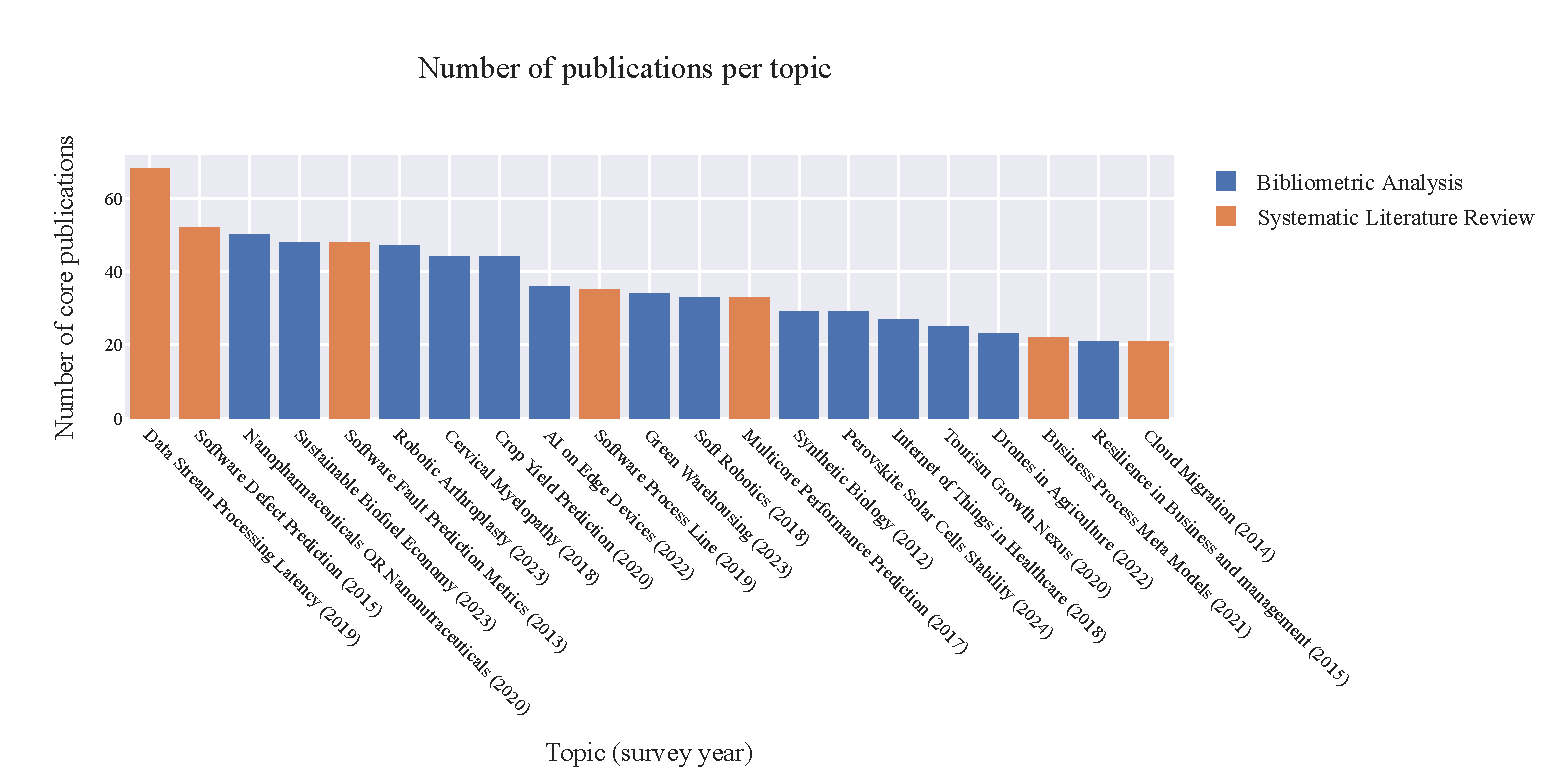
\includegraphics[scale=0.75]{pics/dataset-overview.pdf}
	\caption[Dataset overview of the research topics]{An overview of the dataset and the selected 21 research fields with respective core publications identified through bibliometric analyses or systematic literature review. The number in brackets following the field name on the x-axis represents the year of survey publication.}
	\label{fig:dataset-overview}
\end{figure}


\subsection{Dataset Analysis}

We recognize that potential biases may exist in our dataset due to its complete reliance on the bibliometric community for identifying core publications. This often implies that publications with higher citation counts are deemed more relevant. To assess this, we analyzed the citation distribution per topic, as provided by Dimensions, shown in \autoref{fig:dataset-citation}. Additionally, we examined the distribution of publication years per topic, illustrating the time span considered in the bibliometric analyses, as shown in \autoref{fig:dataset-years}.  If we compare the distribution of publication years for the medical research field \textit{Cervical Myelopathy} with that of \textit{IoT in Healthcare}, both of which were published in 2018, we can observe distinct differences in the year distributions of their core publications. These variations may be attributed to factors such as the recency of the field, changes in terminology over time, or the nature of the research area, where one field may prioritize more established works while the other focuses on recent advancements.


For the evaluation pipeline that we will introduce, the embeddings of the core documents are essential for effectively assessing the search query, as detailed in \autoref{sec:eval-metrics}. To validate this approach, we examine the clustered embeddings of the titles and abstracts for each core topic, as well as the bibliometric analyses in which these documents were initially referenced. This enables us to assess whether core publications within each field exhibit semantic similarity while also demonstrating some degree of dissimilarity from publications in other topics. The resulting clusters, shown in \autoref{fig:dataset-clustering}, were generated using k-means clustering, where $k$ is set to the number of topics. For this, we use OpenAI's small embeddings model alongside t-SNE\autocite{van2008visualizing} to reduce the dimensionality to 2D.

\begin{figure}
	\centering	
	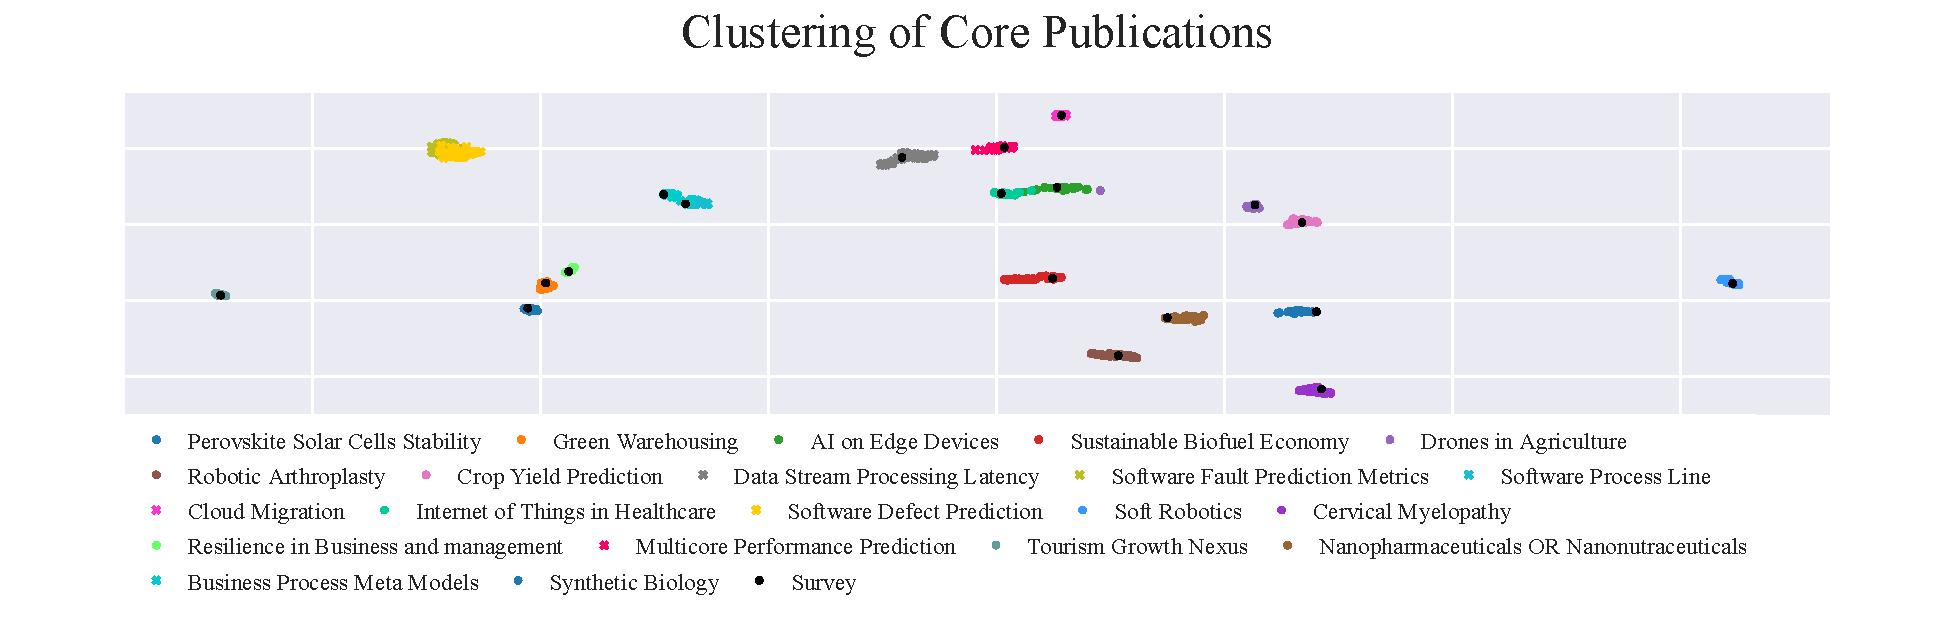
\includegraphics[scale=0.6]{pics/umap_clustering.pdf}
	\caption[Core Publications Clustering]{This figure shows clusters of publication embeddings based on titles and abstracts, the ones marked with o are from the BAs and X from SLRs . Embeddings were generated with OpenAI's small model and reduced in dimensionality with UMAP, then clustered using k-means with $k=21$ (indicating topic count). Clusters group core publications by semantic similarity, with overlaps in topics like \textit{IoT in Healthcare} and \textit{AI on Edge Devices}, as well as most of the SLR topic, due to the similarity in the research field.}
	\label{fig:dataset-clustering}
\end{figure}

\section{Evaluation metrics}\label{sec:eval-metrics}
The standard evaluation metrics for query evaluation are recall and precision. We argue that while recall is of high importance, particularly within the community, precision in this context becomes less feasible. Specifically, retrieving only the exact core publications via a search query would be impractical without explicitly using DOIs to target them directly, which renders this metric largely obsolete and likely to be consistently low. However, we still aim to account for the number of matched publications when executing a search query to prevent models from exploiting overly large queries. To address this, we introduce the concept of \textit{Semantic Precision}.

The idea behind Semantic Precision is to evaluate the relevance of retrieved publications in comparison to the core publication set. If the retrieved publications are sufficiently similar to those in the core set, they are deemed to hold some relevance rather than being entirely unrelated. To achieve this, we assume that the core publications, encompass sufficient semantic breadth to gauge the quality of literature relevant to a specific field. We calculate Semantic Precision in three ways.

\begin{figure}[]
	\centering	
	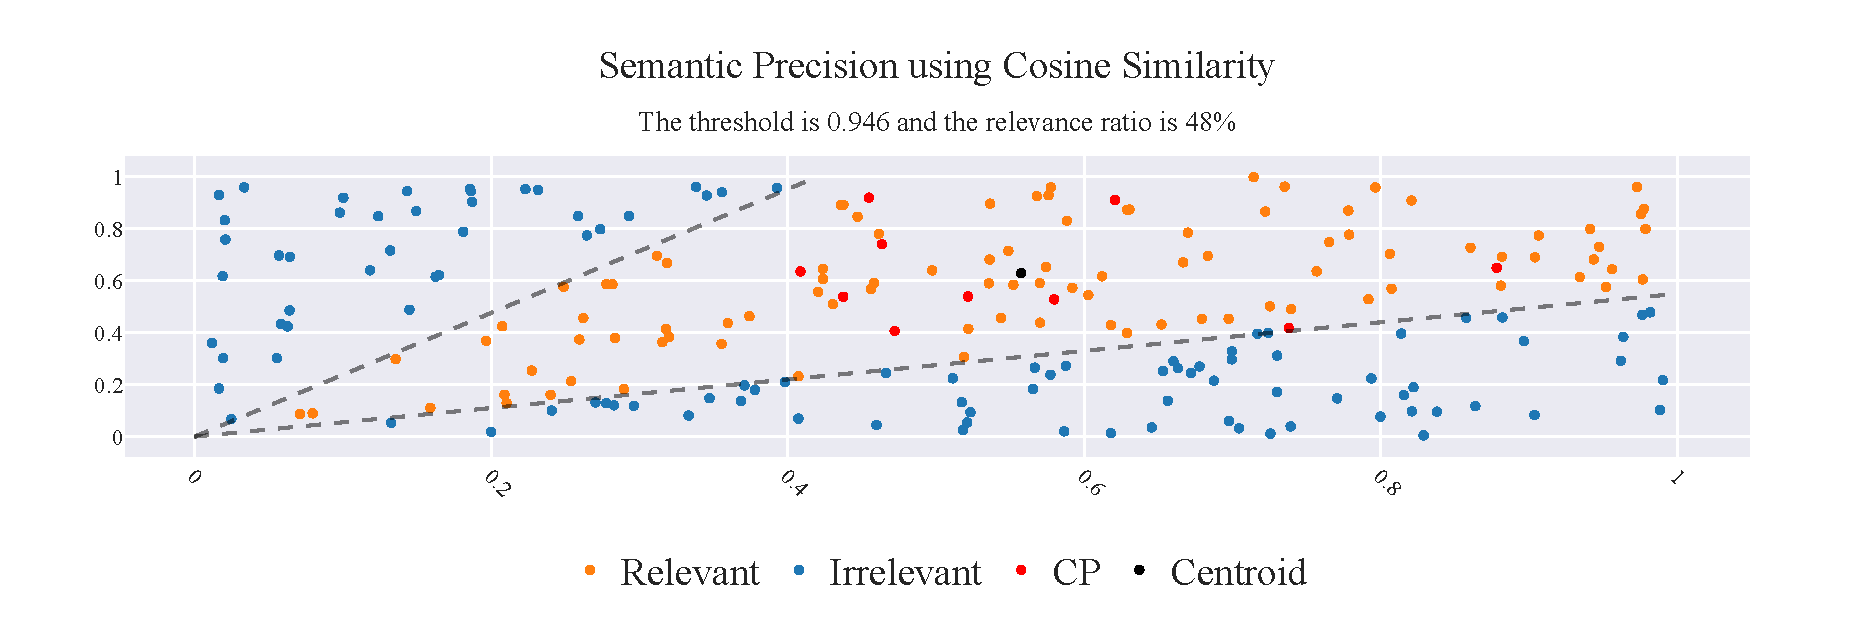
\includegraphics[scale=0.4]{pics/sp_cos.pdf}
	\caption[Semantic Precision using Cosine Similarity]{This illustration demonstrates the effect of cosine similarity on randomly generated data in a 2D space. The core publications (CP) are shown in red, positioned between 0.4 and 0.9 on both the x- and y-axes. When we set the threshold to 0.946, based on the cosine similarity of the least similar core publication from the centroid, many retrieved publications on the opposite side of the spectrum are still assigned as relevant. This effect occurs because cosine similarity considers only the angle between vectors, ignoring their magnitude. In this case, this results in 48\% of the retrieved publications being considered relevant.}

	\label{fig:sp-cos}
\end{figure}

\subsubsection{Semantic Cosine Precision}

The first approach involves averaging the embeddings of the core publications. We then set an acceptance threshold based on the cosine similarity to the least similar core publication, given by. This means that if the embedding of a retrieved publication is more similar to the center than the least similar core publication, we consider it a relevant publication, as shown in \autoref{fig:sp-cos}. We define:
\begin{itemize}
	\item $CPs$ as the set of core publications.
	\item $\vec{c_i}$ as the embedding vector of the $i$-th core publication.
	\item $\vec{p}$ as the embedding vector of a retrieved publication.
	\item $\cos(\vec{a}, \vec{b})$ as the cosine similarity between two vectors $\vec{a}$ and $\vec{b}$.
\end{itemize}

First, compute the centroid of the core publication embeddings:
\[
\vec{c}_{\text{centroid}} = \frac{1}{|CPs|} \sum_{\vec{c_i} \in CPs} \vec{c_i}
\]
Then, let the threshold similarity, $\theta$, be the cosine similarity of the least similar core publication to the centroid:
\[
\theta = \min_{\vec{c_i} \in CP} \cos(\vec{c}_{\text{centroid}}, \vec{c_i})
\]
Finally, Semantic Precision using cosine similarity ($SP_{cos}$) is defined as \autoref{eq:sp-cosine}, where $\mathbb{I}$ is an indicator function that equals 1 if the retrieved publication $\vec{r}$ meets the similarity criterion and 0 otherwise:
\begin{equation}\label{eq:sp-cosine}
	SP_{cos} = \frac{\sum_{\vec{p} \in \text{pubs}} \mathbb{I} \left( \cos(\vec{c}_{\text{centroid}}, \vec{p}) \geq \theta \right)}{|\text{retrieved}|}
\end{equation}

\begin{figure}[h!]
	\centering	
	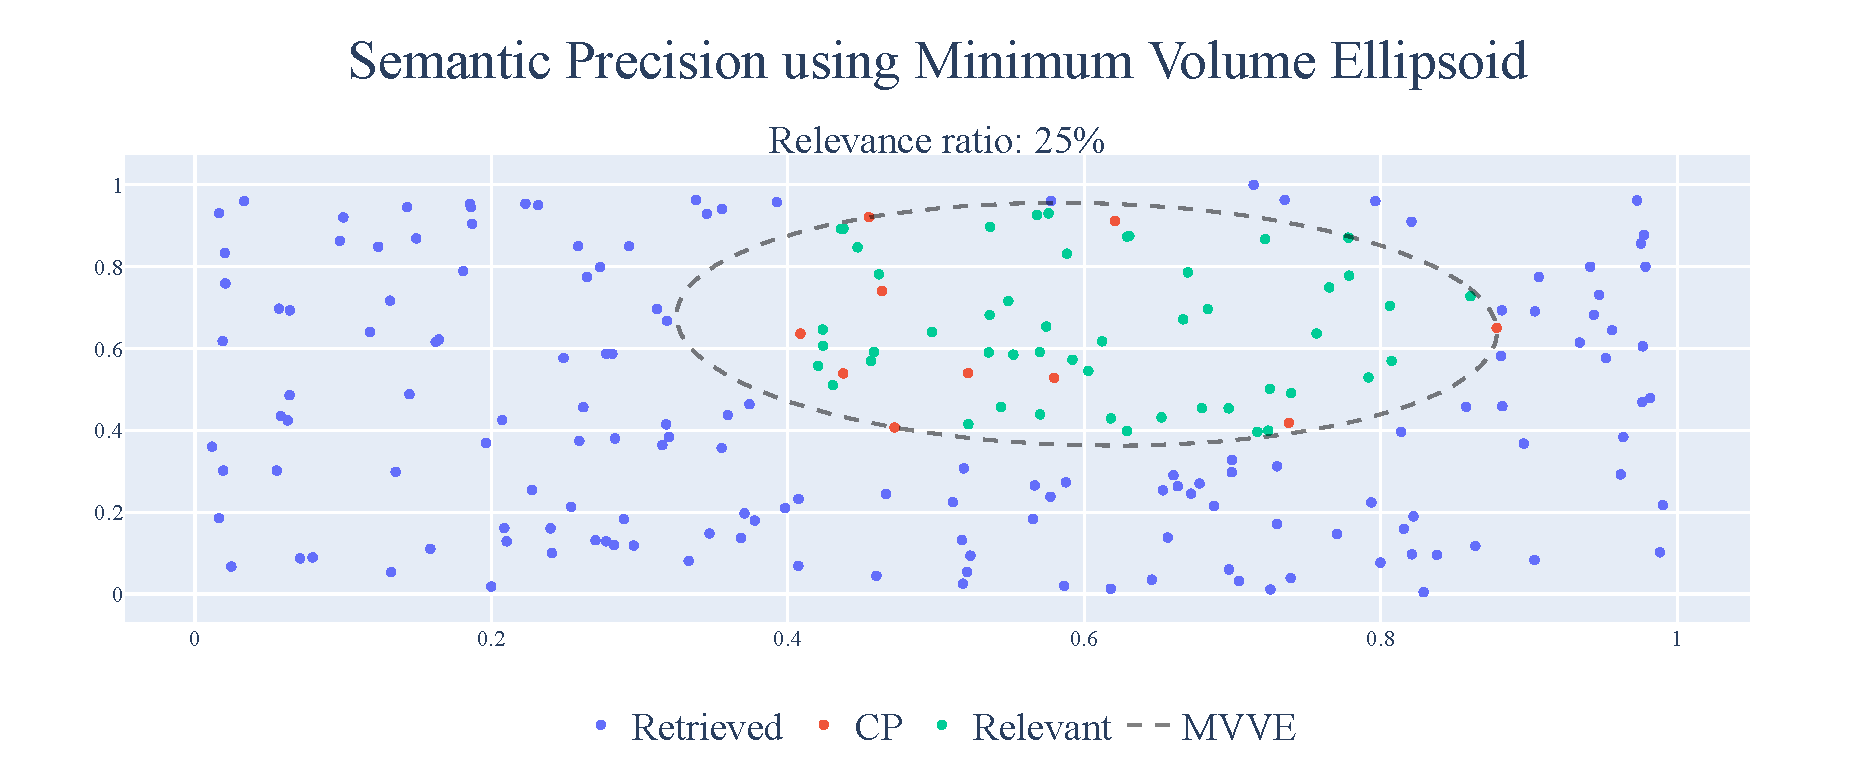
\includegraphics[scale=0.4]{pics/sp_mvee.pdf}
	\caption[Semantic Precision using MVEEE]{This illustration demonstrates the effect of using the Minimum Volume Enclosing Ellipsoid (MVEE) on randomly generated data in a 2D space. The core publications (CP) are shown in red, positioned between 0.4 and 0.9 on both the x- and y-axes. An ellipsoid is generated using MVEE to define the scope of relevant publications, ensuring that only those within the maximal angles and magnitudes of the core publications are considered relevant. In this case, this approach results in only 25\% of the retrieved publications being classified as relevant.}

	\label{fig:sp-mvee}
\end{figure}

\subsubsection{Semantic MVEE Precision}
For the second approach we omit the averaging of the embeddings and use Minimum Volume Enclosing Ellipsoid (MMVE), which creates the smallest ellipsoid that includes the our CP, which we then use to determine which of the retrieved publications are relevant by checking whether they are within MMVE or not, as illustrated in \autoref{fig:sp-mvee}. This approach allows us to take into account all the dimensions by not only considering the angle but also the magnitude

The Minimum Volume Enclosing Ellipsoid (MVEE) for the core publication set $CP$ is centered at $\delta$ with shape matrix $A$. To determine whether a retrieved publication $\vec{r}$ is relevant, we check if it lies within the ellipsoid by testing the following condition:
\[
(\vec{p} - \delta)^T A (\vec{p} - \delta) \leq 1
\]
Semantic Precision (SP) for this approach is then:

\begin{equation}\label{eq:sp-mvee}
	\text{SP}_{\text{MVEE}} = \frac{\sum_{\vec{p} \in \text{pubs}} \mathbb{I} \left( (\vec{p} - \delta)^T A (\vec{p} - \delta) \leq 1 \right)}{|\text{pubs}|}
\end{equation}

Additionally, it is also possible to use a convex hull, which is the smallest convex set that encloses all the points by forming a polygon. A potential advantage of this approach is that it is more robust to outliers compared to the Minimum Volume Enclosing Ellipsoid (MVEE).

\subsubsection{Semantic Clustering Precision}

For the final semantic precision approach, we apply a simple clustering algorithm, such as k-means, on the document embeddings. The process iteratively adjusts the number of clusters \( K \), starting with \( K=2 \), and increases \( K \) until a specific condition is met. We define a threshold \( \theta \) that determines the stopping criterion based on the number of core publications in the smallest cluster. Specifically, we stop when the number of core publications (\( CPs \)) in the smallest cluster satisfies the condition:
\[
CPs \text{ in cluster smallest cluster} \leq \theta \cdot \text{Maximum possible } CPs
\] This ensures that the smallest cluster contains at least \( \theta \) of the core publications.

All the above semantic precision metrics aim to identify potential true positives that were initially not considered as \( CPs \). However, a key issue arises when the number of semantically relevant publications is large due to the broad scope of the initial query. 

For instance, if a query retrieves 50,000 publications, with 30,000 deemed relevant, this still poses a challenge. Screening such a large volume of documents is infeasible, making the results problematic. To address this, we introduce a decay factor to the semantic precision, defined as follows:

\begin{itemize}
	\item \( p \): Controls the initial slowness of the decay.
	\item \( q \): Controls the acceleration of the decay near the end.
	\item $\beta$: The maximum threshold for the decay, representing the point at which the decay becomes negligible.
\end{itemize}

The decay function is expressed as:

\[
\lambda = \left(1 - \left(\frac{n_{\text{pubs}}}{\beta}\right)^p\right)^q
\]


\begin{figure}[h!]
	\centering	
	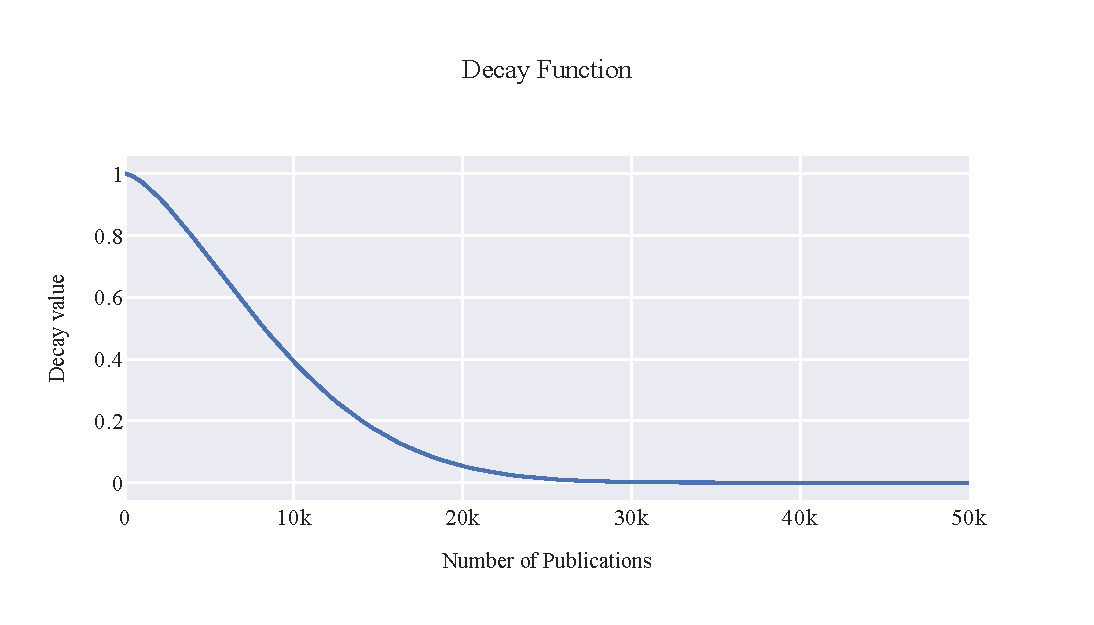
\includegraphics[scale=0.7]{pics/decay_function.pdf}
	\caption[Decay function for semantic precision]{This illustration demonstrates the effect of the decay factor, which ensures that the contribution of a large number of publications diminishes as the total count approaches the threshold. This prevents an overwhelming volume from biasing the semantic precision. For this example, we set the threshold (\( \beta \)) to 50k, \( p=2 \), and \( q=3 \).}	
	\label{fig:decay-function}
\end{figure}


Now that we have metrics that can be used penalizes the model in case of generating a too broad of a query, we use can use it as a factor to calculate the F-Score, the goal of the standard F-score is to balance out between the recall and precision, but in our case we use $F-\beta$ instead, whereby the $\beta$ is the weighting factor of the recall, meaning the higher it is the more important the recall will be, in our case we set it to be 2, meaning that the recall is twice as important as the precision.
\begin{equation}\label{eq:f-beta}
F_\beta = (1 + \beta^2) \cdot \frac{\text{Precision} \cdot \text{Recall}}{(\beta^2 \cdot \text{Precision}) + \text{Recall}}
\end{equation}
For our specific case where $\beta = 2$, emphasizing the importance of recall, it is:
\[
	F_2 = 5 \cdot \frac{(\text{Precision} \cdot \lambda) \cdot \text{Recall}}{(4 \cdot \text{Precision}\cdot \lambda) + \text{Recall}}
\]

\subsection{Comparative Analysis}

To further understand the metrics and their impact on evaluating the dataset, we conduct an in-depth analysis using a randomly selected topic, \textit{Soft Robotics}, as a case study. First, we visualize the embeddings of the baseline and predicted queries \autoref{fig:sr-landscape}. The baseline query is the exact topic name, \textit{Soft Robotics}, while the predicted query is generated by the SQW. The embeddings are derived from the title and abstract of the retrieved publications and subsequently reduced to a 2D UMAP \autocite{mcinnes2020umap} space. It is important to note that a significant amount of information is likely lost due to the extreme dimensionality reduction from 1536 dimensions to 2.


\begin{figure}[!ht]
	\centering	
	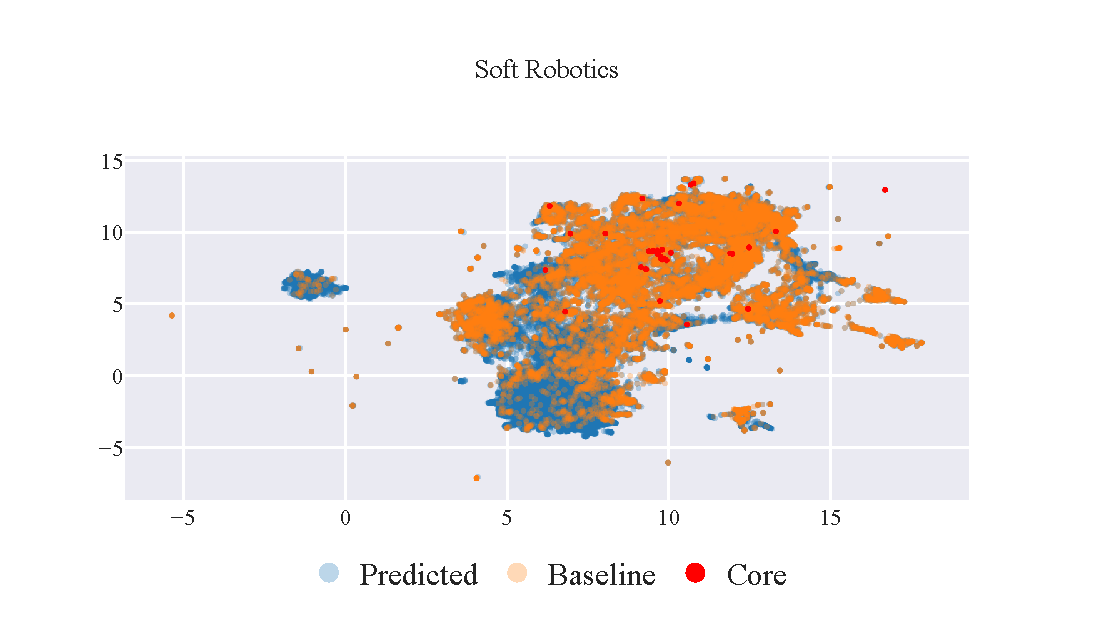
\includegraphics[scale=0.7]{pics/sr-landscape.pdf}
	\caption[Embedding of Soft Robotics]{This figure visualizes the distribution of publications retrieved by both the baseline and predicted queries in a 2D space. The baseline query retrieved 20 core publications, whereas the predicted query retrieved 26 core publications out of a total of 36.}\label{fig:sr-landscape}
\end{figure}

\subsubsection{Semantic Cosine Precision}
At first, we test the Semantic Cosine Precision using the high-dimensional original embedding $E_o$, which was done as described in \autoref{eq:sp-cosine}. This resulted in 13,265 out of 17,573 publications being classified as relevant \autoref{fig:sr-cosine-baseline}. However, this high proportion of relevant publications appeared excessive, prompting further investigation into the threshold's effect on the number of semantically relevant documents.

Since we aim to use the $F_2$ score as our primary evaluation metric, we also employed it as a cost function to maximize. The goal was to identify the optimal empirical threshold that balances the retrieval of core publications with the number of relevant publications. To achieve this, we used the inverse precision, defined as $\frac{\text{Total Retrieved Publications}}{\text{Number of Relevant Publications}}$, instead of standard precision. The results \autoref{fig:threshold-analysis} reveal that a threshold maximizing the number of retrieved core publications while minimizing false positives is approximately 0.69. This suggests that sometimes sacrificing a couple of core publications is rewarding because it allows us to reduce the total number of semantically relevant publications.

\begin{figure}
	\centering	
	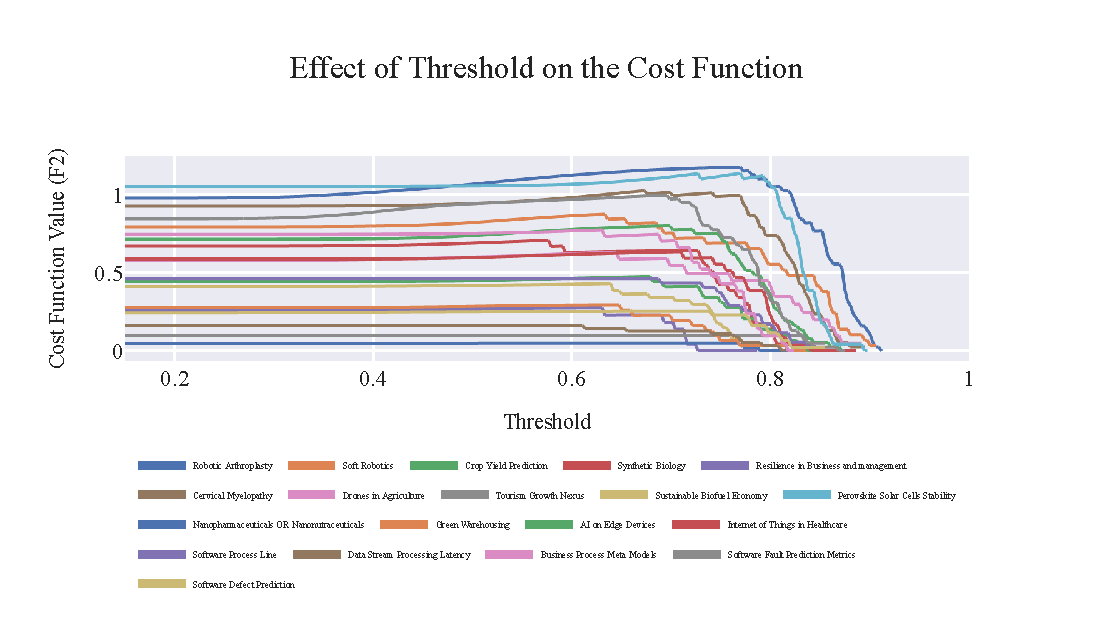
\includegraphics[scale=0.7]{pics/threshold-analysis.pdf}
	\caption[Semantic Cosine Threshold: Empirical Analysis]{This figure illustrates the effect of the threshold on the $F_2$ score. As the threshold increases, the number of semantically relevant publications and core publications identified decreases. However, in some cases, such as \textit{Perovskite Solar Cells Stability}, the $F_2$ score continues to improve despite the loss of a core publication. This outcome is due to the $F_2$ score weighting recall twice as much as precision, allowing for stricter relevance criteria while sacrificing a single core publication.}\label{fig:threshold-analysis}
\end{figure}

After setting the threshold to the optimal empirical value, the Semantic Cosine Precision retrieves 19 out of the initially found 20 core publications while significantly reducing the number of semantically relevant publications by a factor of 4. This adjustment results in only 3,424 publications being identified as relevant, compared to the initial 13,265. However, this refinement comes at the cost of missing one core publication.

\subsubsection{Semantic MVEE Precision}

In contrast to Semantic Cosine Precision, we opt to use the 2D embeddings generated by UMAP $E_{umap}$, rather than the original high-dimensional embeddings, $E_o$. This decision was made because earlier evaluations of the dataset showed that the MVEE consistently classified at least 50\% of the total retrieved documents as relevant, which we believe is related to the high-dimensional nature of the embedding vectors.

We experiment with two enclosing shapes: the MVEE and a Convex Hull. The primary difference is that the MVEE tends to be larger due to its ellipsoidal shape, whereas the convex hull strictly bounds the points. Using the MVEE approach, 9,595 publications were identified as relevant out of the total 17,573 publications, as shown in \autoref{fig:sr-mvee-baseline}. In contrast, the convex hull, being smaller as expected, identified 7,609 publications as relevant, as illustrated in \autoref{fig:sr-hull-baseline}.

\begin{figure}
	\centering	
	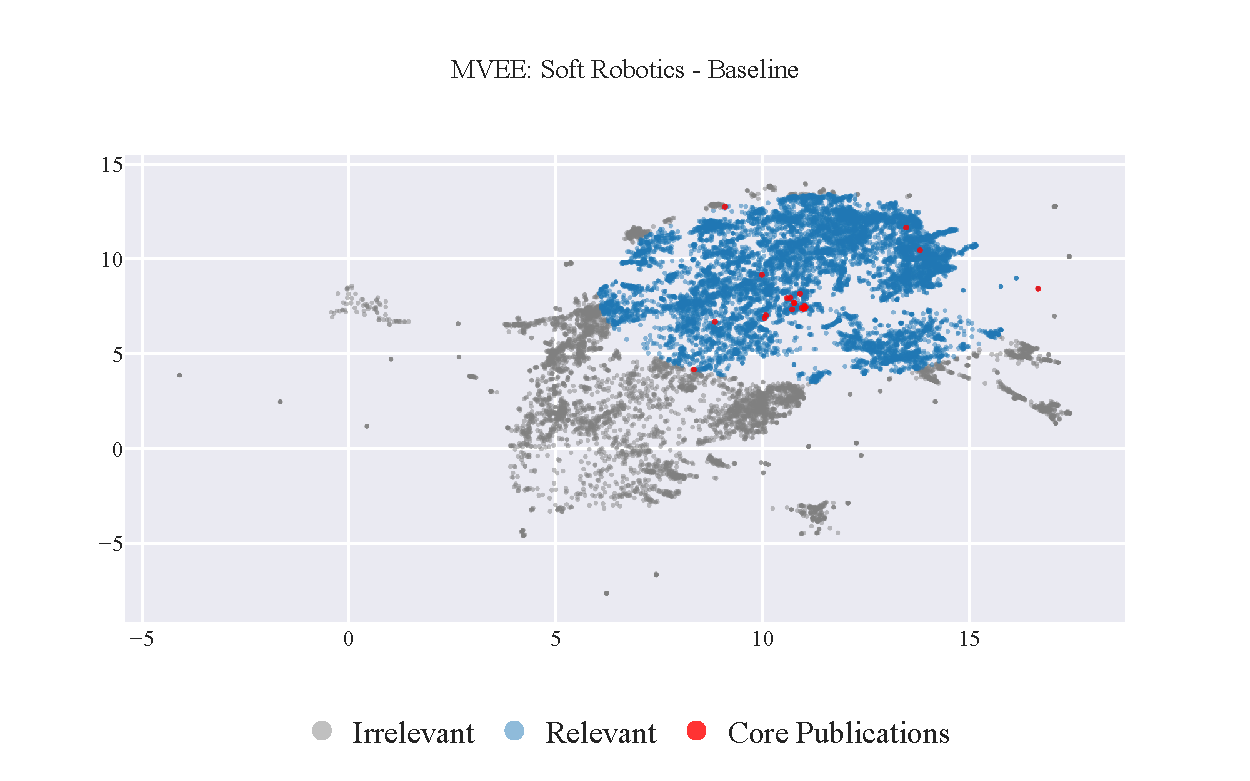
\includegraphics[scale=0.6]{pics/sr-mvee-baseline.pdf}
	\caption[Semantic MVEE Similarity Soft Robotics]{This figure shows the relevant publications identified by the Minimum Volume Enclosing Ellipsoid (MVEE). An advantage of this approach is that we always expect that all teh core publications to be included in the identified publications.}\label{fig:sr-mvee-baseline}
\end{figure}

In the final evaluation, we chose to omit this form of semantic precision due to the reliance on $E_{umap}$, which does not capture the same level of semantic meaning as the higher-dimensional embeddings, $E_o$. Calculating the exact loss of semantic information for UMAP is not straightforward, unlike PCA, which is a linear transformation. However, by employing a Partial Least Squares Regression approach, as described by Oskolkov\footnote{\url{https://towardsdatascience.com/umap-variance-explained-b0eacb5b0801}}, we estimated the explained variance of the two dimensions to be only 7.15\%.

\chapter{Evaluation}\label{ch:eval}
In this section, we evaluate the performance of literature search queries based on the introduced metrics. This evaluation serves as a foundation for developing tools that can potentially generate automatic literature search queries in the future. It is crucial to note that the objective of this evaluation is not to assess the SQW tool itself, but rather to evaluate any arbitrarily generated literature search query. Thus, the focus is solely on the quality of the query, independent of the method by which it was generated.

\section{Experimental Setup}

The curated dataset is constructed using two distinct methods to identify core publications: Bibliometric Analysis (14 topics) and Systematic Literature Review (7 topics), as illustrated in \autoref{fig:dataset-overview}. For the SLRs, the original queries used by the researchers are available. Consequently, we conduct two main experiments. In both experiments we use Dimensions.ai to retrieve all required data. The retrieval process relies on their default relevance-based sorting method, which ranks publications based on the number of keyword matches between the title-abstract and the provided query.

The first experiment involves all 21 topics from both the SLRs and BAs, where we compare a baseline query against a query generated by the SQW. The baseline query consists of the exact topic name, passed into the search engine in a non-exact search fashion. For instance, the query \textit{Soft Robotics} retrieves publications containing both words in their title or abstract, even if they do not appear consecutively.

The predicted query, however, is semi-automatically generated using the SQW tool. This process begins by providing the baseline query as input, which generates a list of keywords. These keywords are then manually sorted by the author into specific or general categories, as described in \autoref{fig:sqw-stage1}. The overarching topic is derived from the topic itself; for example, in the case of \textit{Soft Robotics}, the overarching keyword \textit{Robot} is used. In some cases, the resulting queries produced excessively large results (>100k publications). To address this, keywords were filtered to limit the results to a maximum of 50k publications, balancing evaluation cost and processing speed. Importantly, the baseline query is always included in the predicted query. This ensures that recall is at least as high for the predicted query as for the baseline, making the primary goal of the evaluation to determine whether the expanded query retrieves more core publications than the baseline without becoming overly general by retrieving irrelevant publications.

The second experiment focuses exclusively on the 7 SLR topics. It uses the exact queries and results from the first experiment, but compares them to the SLR queries manually crafted by experts in the field. These expert queries are designed with well-defined research questions aimed at retrieving the most relevant publications that help tackle these exact questions.

\section{Results}
Using the data from the first experiment, we computed all the metrics, namely: Cosine Precision, Clustering Precision, MVEE Precision, Hull Precision, Recall, and the F2 score for each precision metric, as shown in Figure \autoref{fig:all-metrics-1}. When examining the precision metrics, the clustering precision distinctly stands out due to its high value in certain cases, which can be directly attributed to low recall. This recall issue is also evident in some instances for the MVEE and Hull metrics, such as the baseline for \textit{Drones in Agriculture}, where they are set to 0 because fewer than three retrieved core publications are available, which is the minimum number required to define a plane.

A strong correlation is observed between cosine precision and the MVEE and Hull methods, despite relying solely on UMAP embeddings to define the enclosing shapes. This highlights the robustness of these approaches in identifying semantically relevant publications. Additionally, we have two special case topics that had 0 recall, namely \textit{Cloud Migration} and \textit{Multicore Performance Prediction}. As expected, these resulted in a 0 across the board except for the cosine similarity, since it does not require any of the retrieved core publications to exist in order to compute. Instead, it only relies on the pre-computed average embeddings of the core publications. Interestingly, the results for \textit{Cloud Migration} were not considered relevant at all, which we further experimented with and found that the first relevant publication is identified at a threshold of 0.66.


Considering the F2 score, a notable example of the impact of overly large queries without any recall improvement is \textit{Robotic Arthroplasty}. Both the baseline and predicted queries achieved a recall of 0.957, but the expanded predicted query from the SQW retrieved significantly more results overall. Specifically, the predicted query retrieved 22,892 publications, of which only 2,834 were relevant based on cosine similarity. In contrast, the baseline query retrieved 2,151 documents, with 1,904 classified as relevant. This demonstrates how an excessively large query can dilute the precision without improving recall or the number of relevant documents retrieved.

In \autoref{table:expirment-1}, we can better interpret the results of the first experiment by examining the differences between the scores of the predicted query and the baseline. Here, positive values indicate that the predicted query performs better, while negative values show that the baseline outperforms the predicted query. 

As expected, the predicted query consistently achieves similar or better recall across all topics due to the inherent nature of the SQW. However, when evaluating precision, it is evident that the broader queries generated through query expansion often degrade the performance of the model. This effect is particularly visible in the F2 scores, where the increased number of irrelevant publications impacts the balance between recall and precision.

While the SQW demonstrates advantages in terms of recall, its over-expansion often leads to excessive noise in the results. This trade-off is especially clear for topics with a significant drop in precision or F2 scores due to the broader query scope.


\begin{table}
	\caption{In this table we can see the difference in values between the predicted query from the SQW and the baseline, whereby a negative value means that the baseline is better. As anticipated we at least always achieve a similar recall, but in most cases, the SQW yields better recall. However, it severely suffers in precision. When looking at the F2 value, we can see that the tool only notably outperforms the baseline on the three topics \textit{Drones in Agriculture}, \textit{Sustainable Bio Fuel Economy}, and \textit{Multicore Performance Prediction}, whereas it shows a clear disadvantage on the topics \textit{Perovskite Solar Cells Stability}, \textit{Robotic Arthroplasty}, and \textit{Cervical Myelopathy}.}
	\tiny
	\centering
	\hspace*{-1cm}
	\begin{tabular}{p{3cm}c|cccc|cccc}
		& & \multicolumn{4}{c|}{\textbf{Precision}} & \multicolumn{4}{c}{\textbf{F2}} \\ \cline{1-10}
		\multicolumn{1}{c}{\centering \textbf{Topic}} &
		\multicolumn{1}{p{1cm}|}{\centering \textbf{Recall}} &
		\multicolumn{1}{p{0.8cm}}{\centering \textbf{Cosine}} &
		\multicolumn{1}{p{1.2cm}}{\centering \textbf{Clustering}} & 
		\multicolumn{1}{p{0.8cm}}{\centering \textbf{MVEE}} & 
		\multicolumn{1}{p{0.8cm}|}{\centering \textbf{Hull}} & 
		\multicolumn{1}{p{0.8cm}}{\centering \textbf{Cosine}} & 
		\multicolumn{1}{p{1.2cm}}{\centering \textbf{Clustering}} & 
		\multicolumn{1}{p{0.8cm}}{\centering \textbf{MVEE}}  & 
		\multicolumn{1}{p{0.8cm}}{\centering \textbf{Hull}}  \\ \hline 
		\centering{Robotic Arthroplasty} & 0.000 &  -0.761 &  -0.528 &  -0.707 &  -0.679 &  -0.560 &  -0.490 &  -0.570 &  -0.570 \\
		\centering{Soft Robotics} & \textbf{0.111} &  -0.134 &  -0.147 &  -0.292 &  -0.152 &  -0.130 &  -0.090 &  -0.400 &  -0.300 \\
		\centering{Crop Yield Prediction} & \textbf{0.109} &  -0.280 &  -0.118 &  -0.261 &  -0.234 &  -0.210 &  -0.230 &  -0.740 &  -0.530 \\
		\centering{Synthetic Biology} & \textbf{0.310} &  -0.050 &  -0.185 & \textbf{0.637} & \textbf{0.510} & \textbf{0.030} & \textbf{0.080} &  -0.420 &  -0.330 \\
		\centering{Resilience in Business and management} & \textbf{0.185} &  -0.022 &  -0.838 & \textbf{0.150} & \textbf{0.071} & \textbf{0.060} & \textbf{0.170} & \textbf{0.330} & \textbf{0.240} \\
		\centering{Cervical Myelopathy} & \textbf{0.085} &  -0.298 &  -0.299 &  -0.061 &  -0.017 &  -0.330 &  -0.250 &  -0.700 &  -0.590 \\
		\centering{Drones in Agriculture} & \textbf{0.480} &  -0.184 & \textbf{0.298} & \textbf{0.069} & \textbf{0.028} & \textbf{0.220} & \textbf{0.160} & \textbf{0.240} & \textbf{0.120} \\
		\centering{Tourism Growth Nexus} & 0.000 &  -0.562 & \textbf{0.310} & 0.000 & 0.000 &  -0.070 &  -0.040 & 0.000 & 0.000 \\
		\centering{Sustainable Biofuel Economy} & \textbf{0.260} &  -0.122 & \textbf{0.733} & \textbf{0.513} & \textbf{0.343} & \textbf{0.190} & 0.000 & \textbf{0.150} & \textbf{0.320} \\
		\centering{Perovskite Solar Cells Stability} & \textbf{0.103} &  -0.237 &  -0.213 & \textbf{0.051} & \textbf{0.082} &  -0.460 &  -0.430 &  -0.470 &  -0.540 \\
		\centering{Nanopharmaceuticals OR Nanonutraceuticals} & \textbf{0.040} & \textbf{0.003} &  -0.376 & 0.000 & 0.000 & \textbf{0.040} & \textbf{0.010} & 0.000 & 0.000 \\
		\centering{Green Warehousing} & \textbf{0.052} &  -0.227 &  -0.411 & \textbf{0.023} & \textbf{0.004} &  -0.130 &  -0.030 &  -0.530 &  -0.200 \\
		\centering{AI on Edge Devices} & \textbf{0.250} &  -0.227 & \textbf{0.050} & \textbf{0.182} & \textbf{0.138} & \textbf{0.090} &  -0.090 &  -0.050 & \textbf{0.200} \\
		\centering{Internet of Things in Healthcare} & \textbf{0.172} &  -0.203 &  -0.090 &  -0.146 &  -0.109 &  -0.050 &  -0.160 &  -0.500 &  -0.400 \\
		\centering{Software Process Line} & \textbf{0.024} &  -0.001 & \textbf{0.239} &  -0.048 &  -0.037 & 0.000 &  -0.020 &  -0.660 &  -0.300 \\
		\centering{Data Stream Processing Latency} & \textbf{0.087} &  -0.292 &  -0.480 &  -0.237 &  -0.196 &  -0.130 &  -0.150 &  -0.510 &  -0.480 \\
		\centering{Business Process Meta Models} & \textbf{0.307} &  -0.199 &  -0.233 &  -0.228 &  -0.148 &  -0.090 &  -0.050 &  -0.360 &  -0.300 \\
		\centering{Multicore Performance Prediction} & \textbf{0.273} &  -0.239 & 0.000 & \textbf{0.158} & \textbf{0.100} & \textbf{0.200} & \textbf{0.010} & \textbf{0.400} & \textbf{0.320} \\
		\centering{Cloud Migration} & 0.000 & 0.000 & 0.000 & 0.000 & 0.000 & 0.000 & 0.000 & 0.000 & 0.000 \\
		\centering{Software Fault Prediction Metrics} & \textbf{0.312} &  -0.604 & \textbf{0.671} & \textbf{0.006} & \textbf{0.012} &  -0.050 & \textbf{0.020} &  -0.090 &  -0.010 \\
		\centering{Software Defect Prediction} & \textbf{0.186} &  -0.466 &  -0.311 &  -0.121 &  -0.233 &  -0.040 & \textbf{0.030} &  -0.390 &  -0.300 \\
	\end{tabular}\label{table:expirment-1}
\end{table}


The results of the second experiment, which compare the actual search queries used to identify the core publications in the SLRs, have yielded surprising yet explainable outcomes. It is important to re-emphasize that the queries initially used for the SLRs were adapted to fit dimension's query criteria and were only applied to search the title and abstract. In contrast, the original queries were utilized across a variety of search indices, such as title, abstract, full text, and sometimes full data for specific fields, which is a form query fine-tuning that is search engine specific. Therefore, it is important to note that the results will always be search engine dependent, which, in this case, is dimensions.ai.

As shown in \autoref{fig:all-metrics-2}, the results of the SLR queries are not as anticipated, particularly since they were expected to yield high recall. This discrepancy arises from the queries' reconstruction and adaptation to fit dimensions' criteria. The performance difference between the SLR queries and the baseline can be observed in \autoref{table:expirment-2}. Overall, the baseline and the SLR queries performed on nearly equal footing, with two topics favoring the SLR and three favoring the baseline. 

Interestingly, in case where the recall of the baseline significantly outperformed the SLR, namely \textit{Software Fault Prediction Metrics}, the cosine precision was drastically lower. This results in an unwanted behavior which can be interpreted by the cosine-F2 score being 0, indicating that the recall gain was of no value due to the excessive number of irrelevant retrieved publications.

\begin{table}
	\caption{This table displays the differences in values between the predicted query from the SLR and the baseline, where a negative value indicates that the baseline performs better.}
	\tiny
	\centering
	\hspace*{-1cm}
	\begin{tabular}{p{3cm}c|cccc|cccc}
		& & \multicolumn{4}{c|}{\textbf{Precision}} & \multicolumn{4}{c}{\textbf{F2}} \\ \cline{1-10}
		\multicolumn{1}{c}{\centering \textbf{Topic}} &
		\multicolumn{1}{p{1cm}|}{\centering \textbf{Recall}} &
		\multicolumn{1}{p{0.8cm}}{\centering \textbf{Cosine}} &
		\multicolumn{1}{p{1.2cm}}{\centering \textbf{Clustering}} & 
		\multicolumn{1}{p{0.8cm}}{\centering \textbf{MVEE}} & 
		\multicolumn{1}{p{0.8cm}|}{\centering \textbf{Hull}} & 
		\multicolumn{1}{p{0.8cm}}{\centering \textbf{Cosine}} & 
		\multicolumn{1}{p{1.2cm}}{\centering \textbf{Clustering}} & 
		\multicolumn{1}{p{0.8cm}}{\centering \textbf{MVEE}}  & 
		\multicolumn{1}{p{0.8cm}}{\centering \textbf{Hull}}  \\ \hline 
		\centering{Software Process Line} &  -0.232 & \textbf{0.286} & \textbf{0.319} & \textbf{0.162} & \textbf{0.194} & \textbf{0.250} & \textbf{0.140} & \textbf{0.290} & \textbf{0.360} \\
		\centering{Data Stream Processing Latency} &  -0.073 &  -0.008 &  -0.321 &  -0.157 &  -0.125 &  -0.070 &  -0.100 &  -0.160 &  -0.160 \\
		\centering{Business Process Meta Models} & \textbf{0.269} & \textbf{0.039} &  -0.082 & \textbf{0.421} & \textbf{0.281} & \textbf{0.190} & \textbf{0.090} & \textbf{0.390} & \textbf{0.390} \\
		\centering{Multicore Performance Prediction} & 0.000 & \textbf{0.217} & 0.000 & 0.000 & 0.000 & 0.000 & 0.000 & 0.000 & 0.000 \\
		\centering{Cloud Migration} & 0.000 & 0.000 & 0.000 & 0.000 & 0.000 & 0.000 & 0.000 & 0.000 & 0.000 \\
		\centering{Software Fault Prediction Metrics} & \textbf{0.562} &  -0.596 & \textbf{0.061} & \textbf{0.005} & 0.000 & 0.000 & \textbf{0.330} &  -0.040 &  -0.020 \\
		\centering{Software Defect Prediction} &  -0.129 &  -0.584 &  -0.446 &  -0.619 &  -0.491 &  -0.280 &  -0.210 &  -0.750 &  -0.750 \\
	\end{tabular}\label{table:expirment-2}
\end{table}

\section{Discussion}

The primary goal of this work was to determine the quality of literature search queries, emphasizing recall, which is widely regarded as an essential measure in the research community. However, precision has historically been less emphasized due to the intrinsic nature of literature search queries, which tend to favor comprehensiveness over specificity. By developing multiple metrics to evaluate the relevance of publications in a semantic space, we successfully integrated precision into the evaluation framework by introducing semantic precision.

To calculate semantic precision, we employed four metrics: semantic cosine, clustering, MVEE, and Hull precision. Each metric demonstrated distinct advantages and limitations. Initially, we hypothesized that the cosine similarity threshold should correspond to the least similar core publication. However, in certain cases, sacrificing a core publication to substantially reduce the number of irrelevant publications proved more beneficial in terms of the F2 score. Consequently, we adopted an empirical threshold estimated by maximizing the F2 score across all topics.

For Convex Hull and MVEE, we first tested their performance using the original embeddings in their high-dimensional space. However, these metrics consistently overestimated precision, often exceeding 50\%. This discrepancy is likely due to the curse of dimensionality, which complicates the construction of accurate ellipsoids or hulls in high-dimensional spaces, possibly reflecting limitations in the embedding construction process. This observation led to the decision to switch to UMAP embeddings, which offer a reduced dimensionality and improved computational feasibility. However, while UMAP embeddings show potential, the exact amount of semantic value lost compared to the original high-dimensional embeddings remains unclear.

A common issue for clustering, MVEE, and Hull methods lies in their dependency on recall. Semantic clustering requires at least two core publications, and performance improves with more core publications as the clustering process narrows the focus on relevant publications. This limitation becomes problematic when the viable core publications count is less than two. Similarly, MVEE and Hull methods necessitate at least three core publications to construct a plane capable of enclosing other potentially relevant publications. In contrast, cosine similarity only requires the pre-computed mean embedding of the core publications and a similarity threshold. This independence from recall allows cosine similarity to determine relevance even when recall is minimal, making it a more robust metric in cases of sparse core publications.






{\let\clearpage\relax \chapter{Conclusion}\label{ch:conclusion}}

\section{Summary and Contributions}
This work presents \textbf{LitQEval}, a novel framework addressing limitations in evaluating literature search query generation. Existing datasets like CLEF and Collection of Seeds often focus on medical data, and while more diverse datasets like Badami’s \autocite{badami2023adaptive} exist, they lack robust evaluation metrics. The primary issues identified are the overemphasis on recall at the expense of precision and the problem of overly broad queries generating excessive irrelevant results. 

LitQEval introduces a more comprehensive dataset covering 21 diverse topics. Core publications were collected using bibliometric analyses and SLRs to ensure relevance. The dataset is validated using techniques like clustering embeddings of publication titles and abstracts, confirming semantic similarity within fields while distinguishing between different topics.

New evaluation metrics are proposed to balance recall and precision. \textit{Semantic Precision} evaluates the relevance of retrieved publications compared to core publications through four approaches: (1) Cosine Similarity, (2) Minimum Volume Enclosing Ellipsoid, (3) Convex Hull and (4) Clustering. These metrics aim to determine relevant publications retrieved by queries via semantic similarity. A decay factor further adjusts precision to account for query breadth.

To balance recall and precision, the \textit{ F-$2$ } score emphasizes recall for evaluating queries. Comparative analyses, including a case study on "Soft Robotics," validate the metrics, revealing insights into the trade-offs between core publication retrieval and query specificity.

Overall, we recommend the \textbf{Cosine Precision} as a default metric, as it does not require any CPs to be retrieved by the query for evaluation and becomes more robust as the number of retrieved CPs increases. However, in cases where the number of CPs retrieved falls between 3 and 10, Hull Precision could also be useful, as the number of potential relevant publications remains small enough to avoid negatively affecting the F2 score.

The dataset and code used in this work are publicly available in the LitQEval repository\footnote{\url{https://github.com/Mohammadsaknini/LitQEval}} on GitHub.

\section{Outlook}
This effort forms part of a broader initiative, the SQW, developed by Fraunhofer INT. The SQW aims to automate or semi-automate the creation of literature queries, expediting research on emerging topics and offering researchers a quick starting point. While this study concentrated on building a pipeline for evaluating search queries rather than testing SQW's performance, numerous opportunities remain to enhance the tool. These include using the second step, \textit{Iterative Scientific Fine-Tuning}, to refine results further. Additionally, testing optional inputs such as detailed descriptions, uploads of relevant publications, or adjusting model parameters (e.g., temperature for exploration) holds significant potential for improvement.

Beyond the SQW, the framework for evaluating query quality introduces new opportunities. For instance, it facilitates the creation of scientific chatbots capable of answering complex questions by combining standard queries, research questions, or relevant publications as inputs. Such tools could use cosine similarity within a large semantic space to identify and retrieve additional relevant publications effectively.

This study highlights several promising directions for future research and development. One key avenue is the refinement and broader application of the semantic precision metrics introduced here. For instance, future work could explore how to adapt these metrics to dynamic and interdisciplinary research areas where core publications may be less clearly defined. 

Lastly, the broader implications of this work in developing AI-driven research tools warrant continued exploration. From advanced literature search engines to domain-specific scientific assistants, the principles established here could inform the next generation of tools designed to augment and streamline academic research workflows.
\appendix

\chapter{Appendix}

\begin{figure}[!h]
	\centering	
	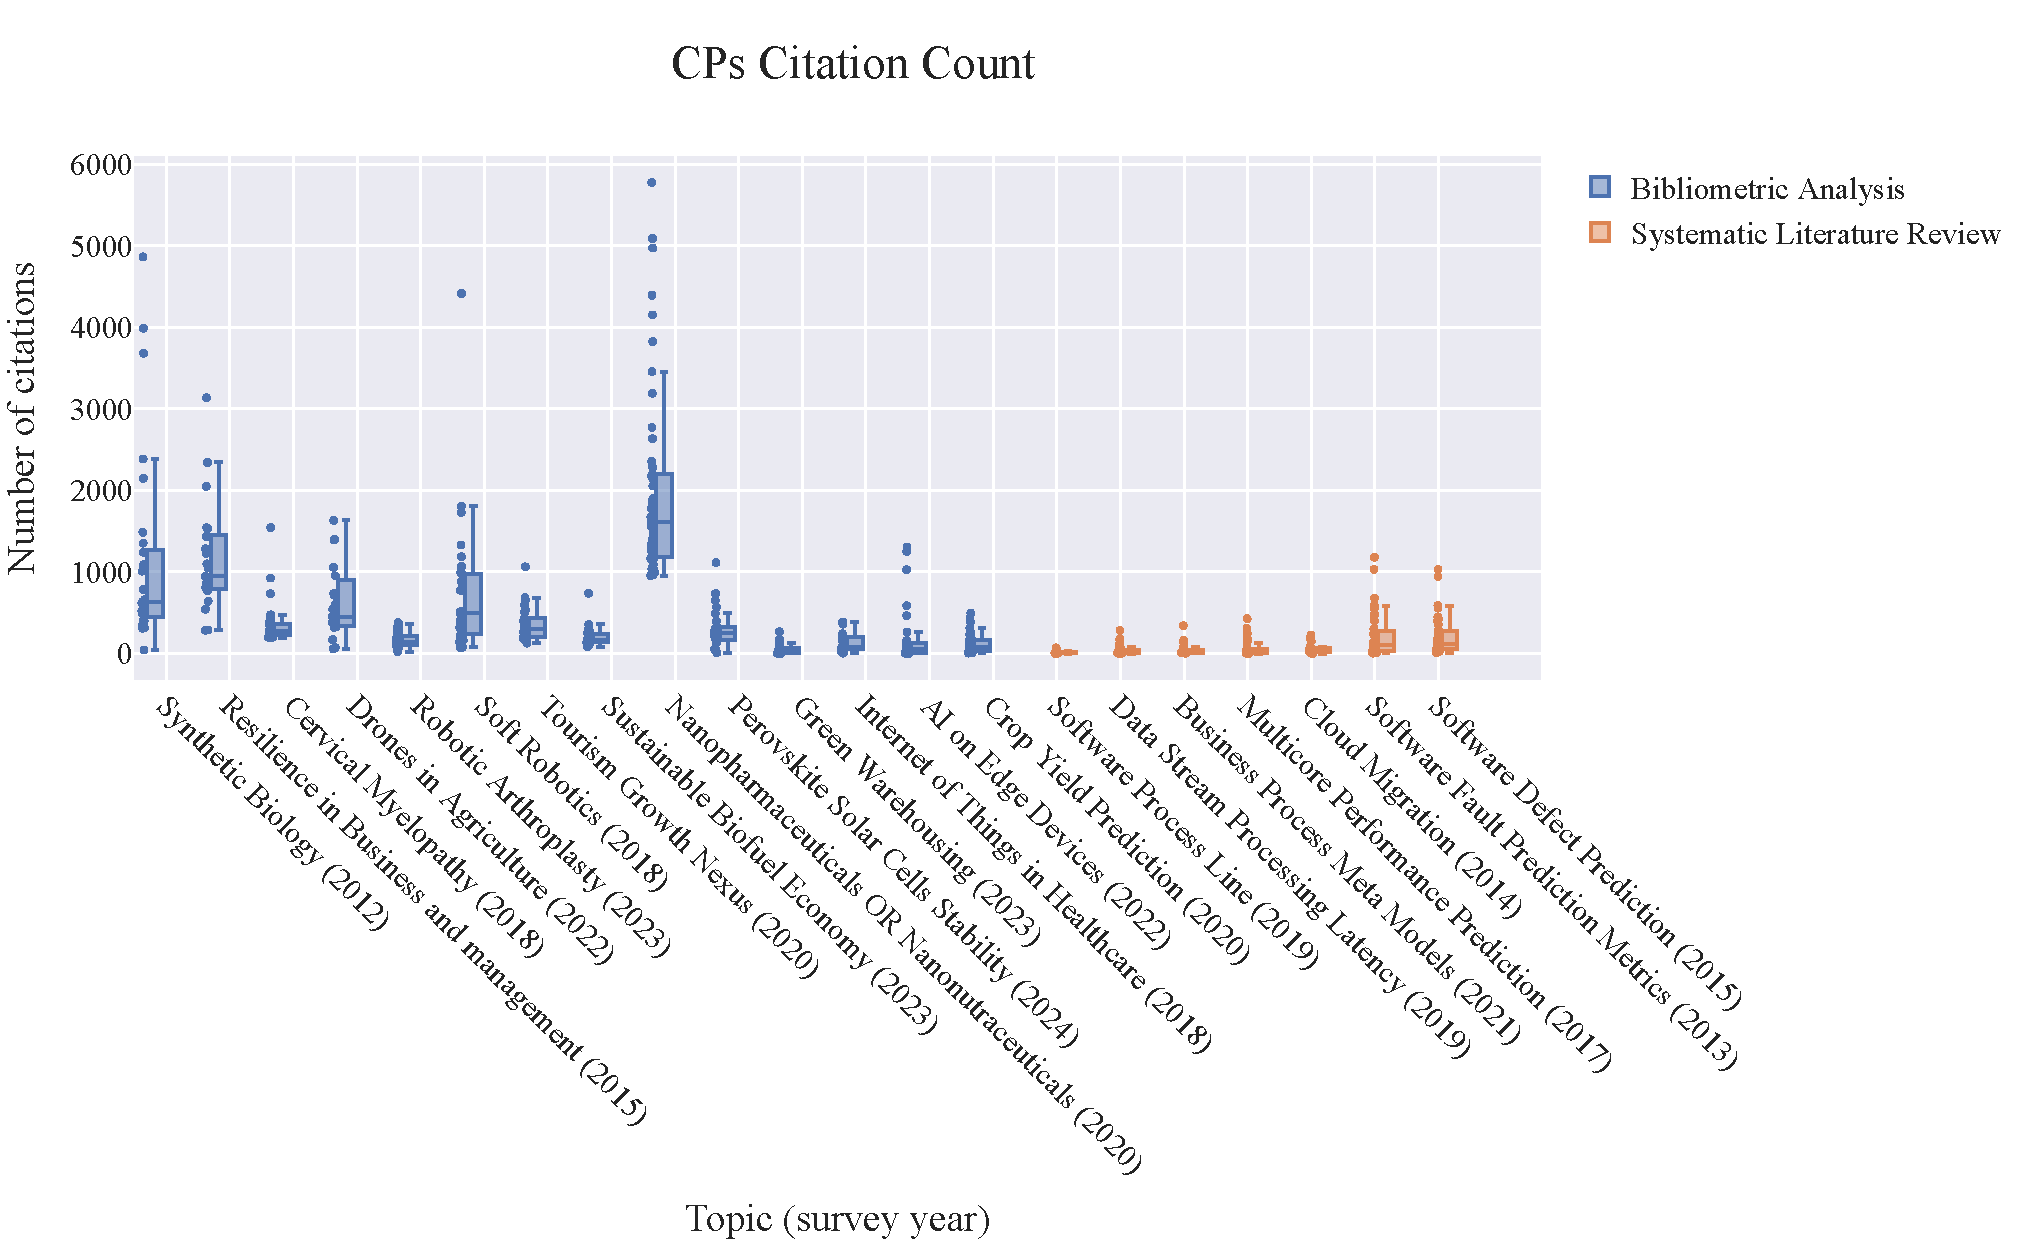
\includegraphics{pics/citation-distribution.pdf}
	\caption[Field Citation Ratio per Topic]{The citation ratio per topic, showing the relative citation counts of core publications compared to the average citation frequency within their respective research fields. This illustrates how the prominence of each publication compares to typical citation levels in its field.}
	\label{fig:dataset-citation}
\end{figure}

\begin{figure}
	\centering	
	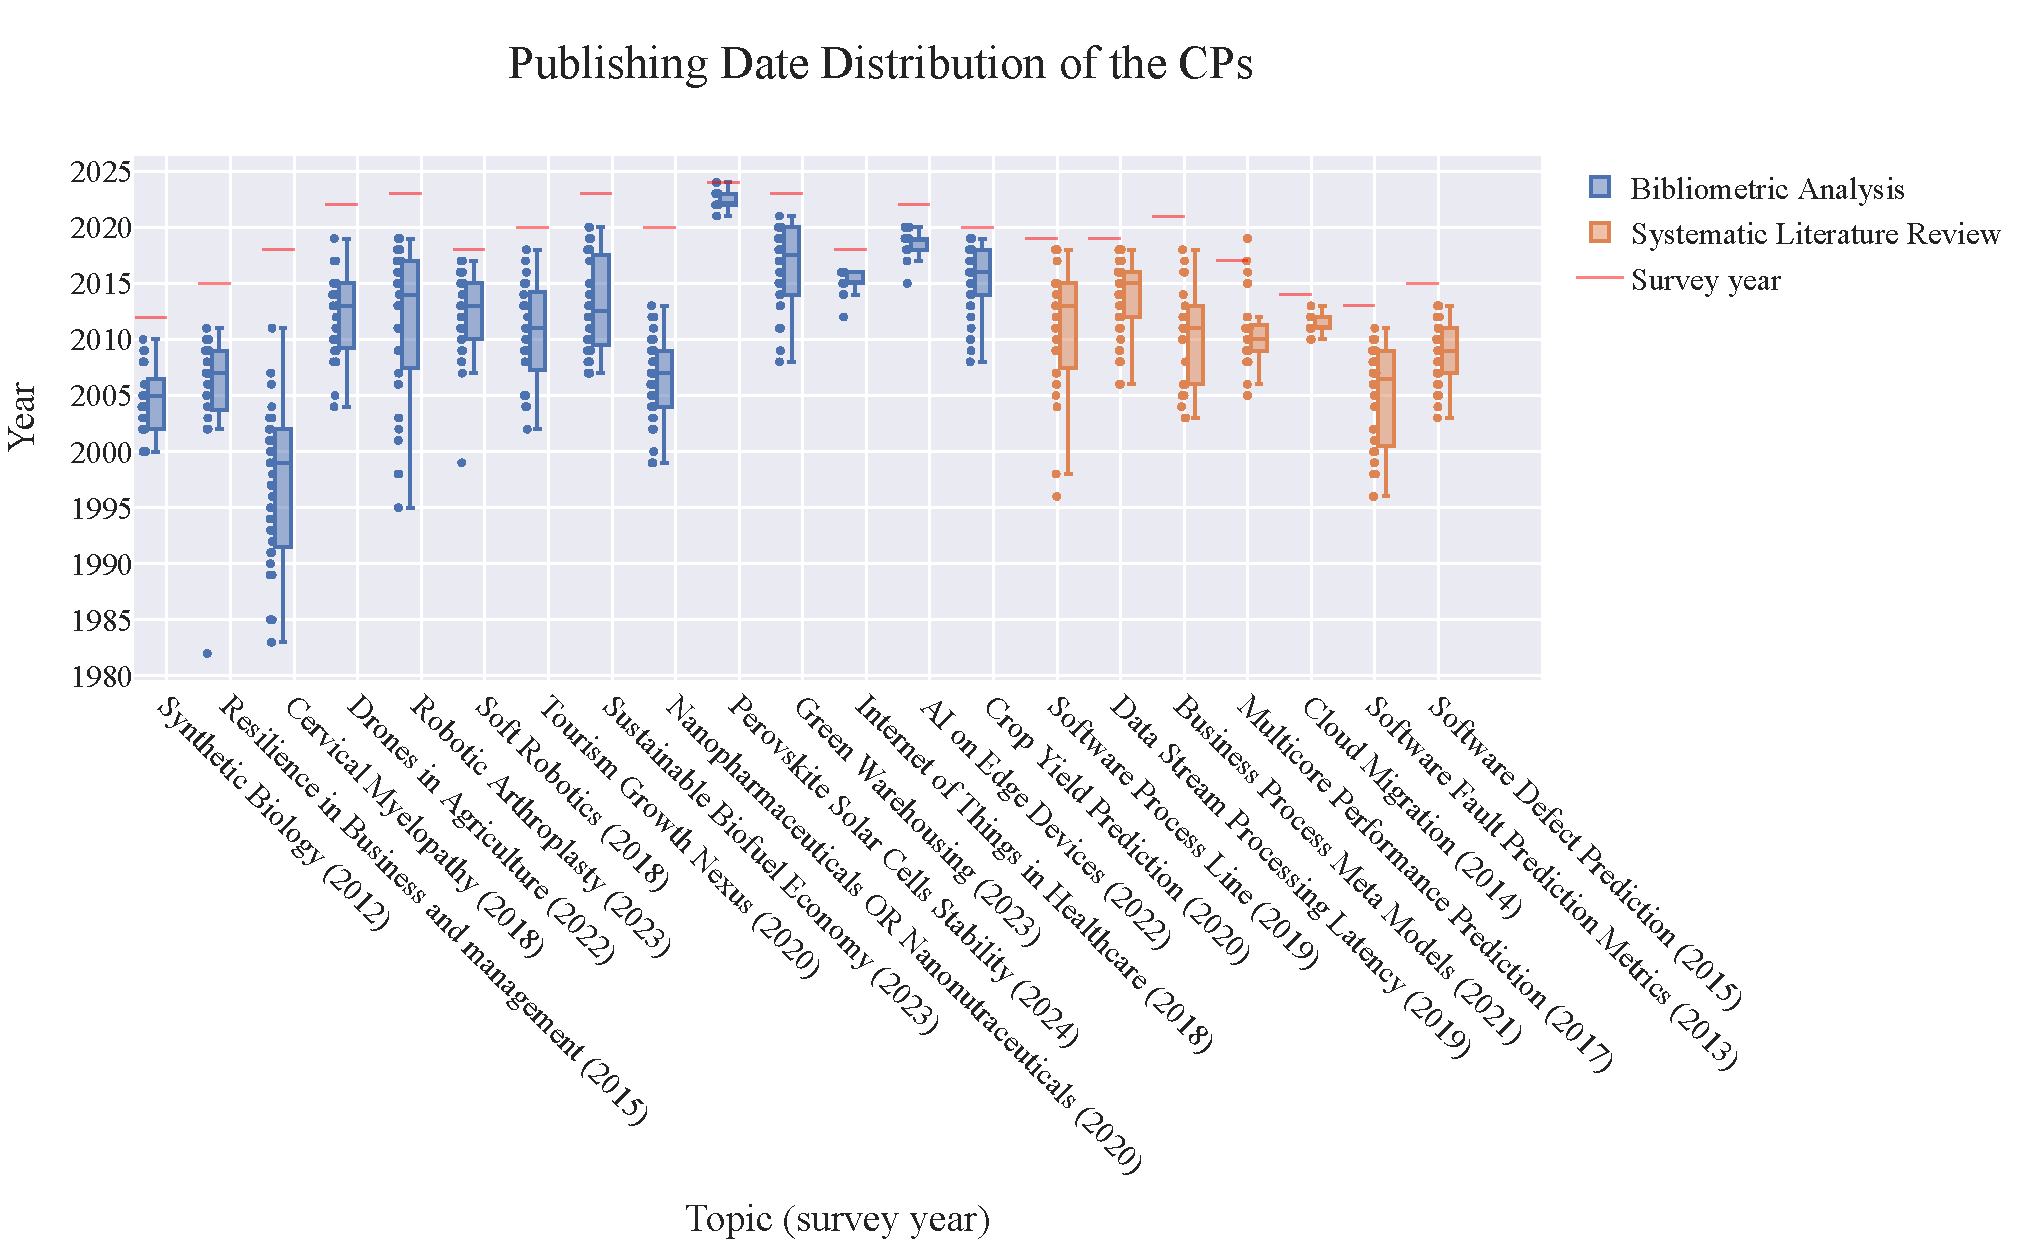
\includegraphics{pics/year-distribution.pdf}
	\caption[Distribution of publication years per topic]{The distribution of publication years for core publications across various research topics, highlighting the historical range of studies considered in the bibliometric analyses for each field. Notably, for \textit{Cervical Myelopathy}, the lower bound of publication years was set to 1980 for improved readability, although the actual range goes back to 1953.}
	\label{fig:dataset-years}
\end{figure}

\begin{figure}
	\centering	
	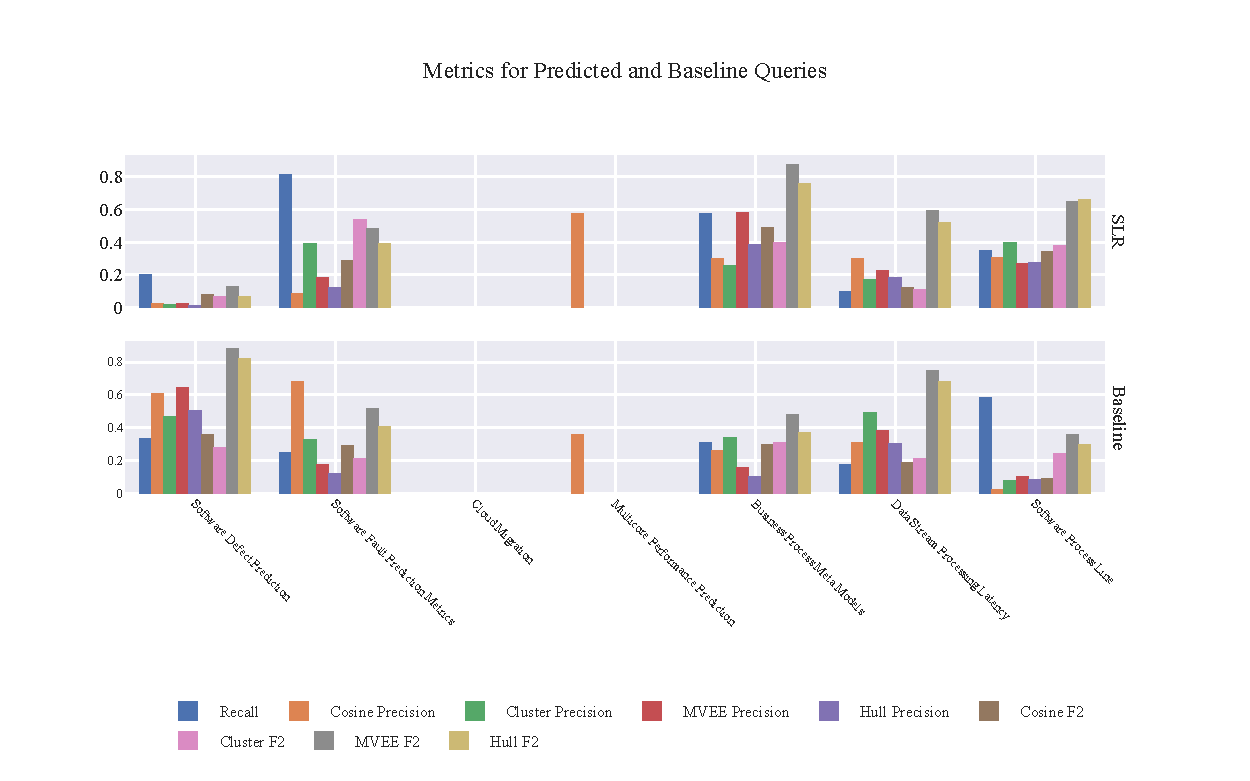
\includegraphics[scale=0.7]{pics/all-metrics-2.pdf}
	\caption[Evaluation: Experiment 2]{This figure shows the results of the second experiment across all the SLR datasets. Surprisingly, we can see that using the SLR query does not achieve outstanding results, which is attributed to its reconstruction and adaptation to fit dimension's search engine. Notably, issues similar to those from the first experiment due to the recall of 0 are also apparent in this case. Notably, the SLR query used for \textit{Multicore Performance Prediction} is only partially available for public access \autocite{Frank2017}, hence the very low scores.}\label{fig:all-metrics-2}
\end{figure}

\begin{figure}
	\hspace*{-4cm}	
	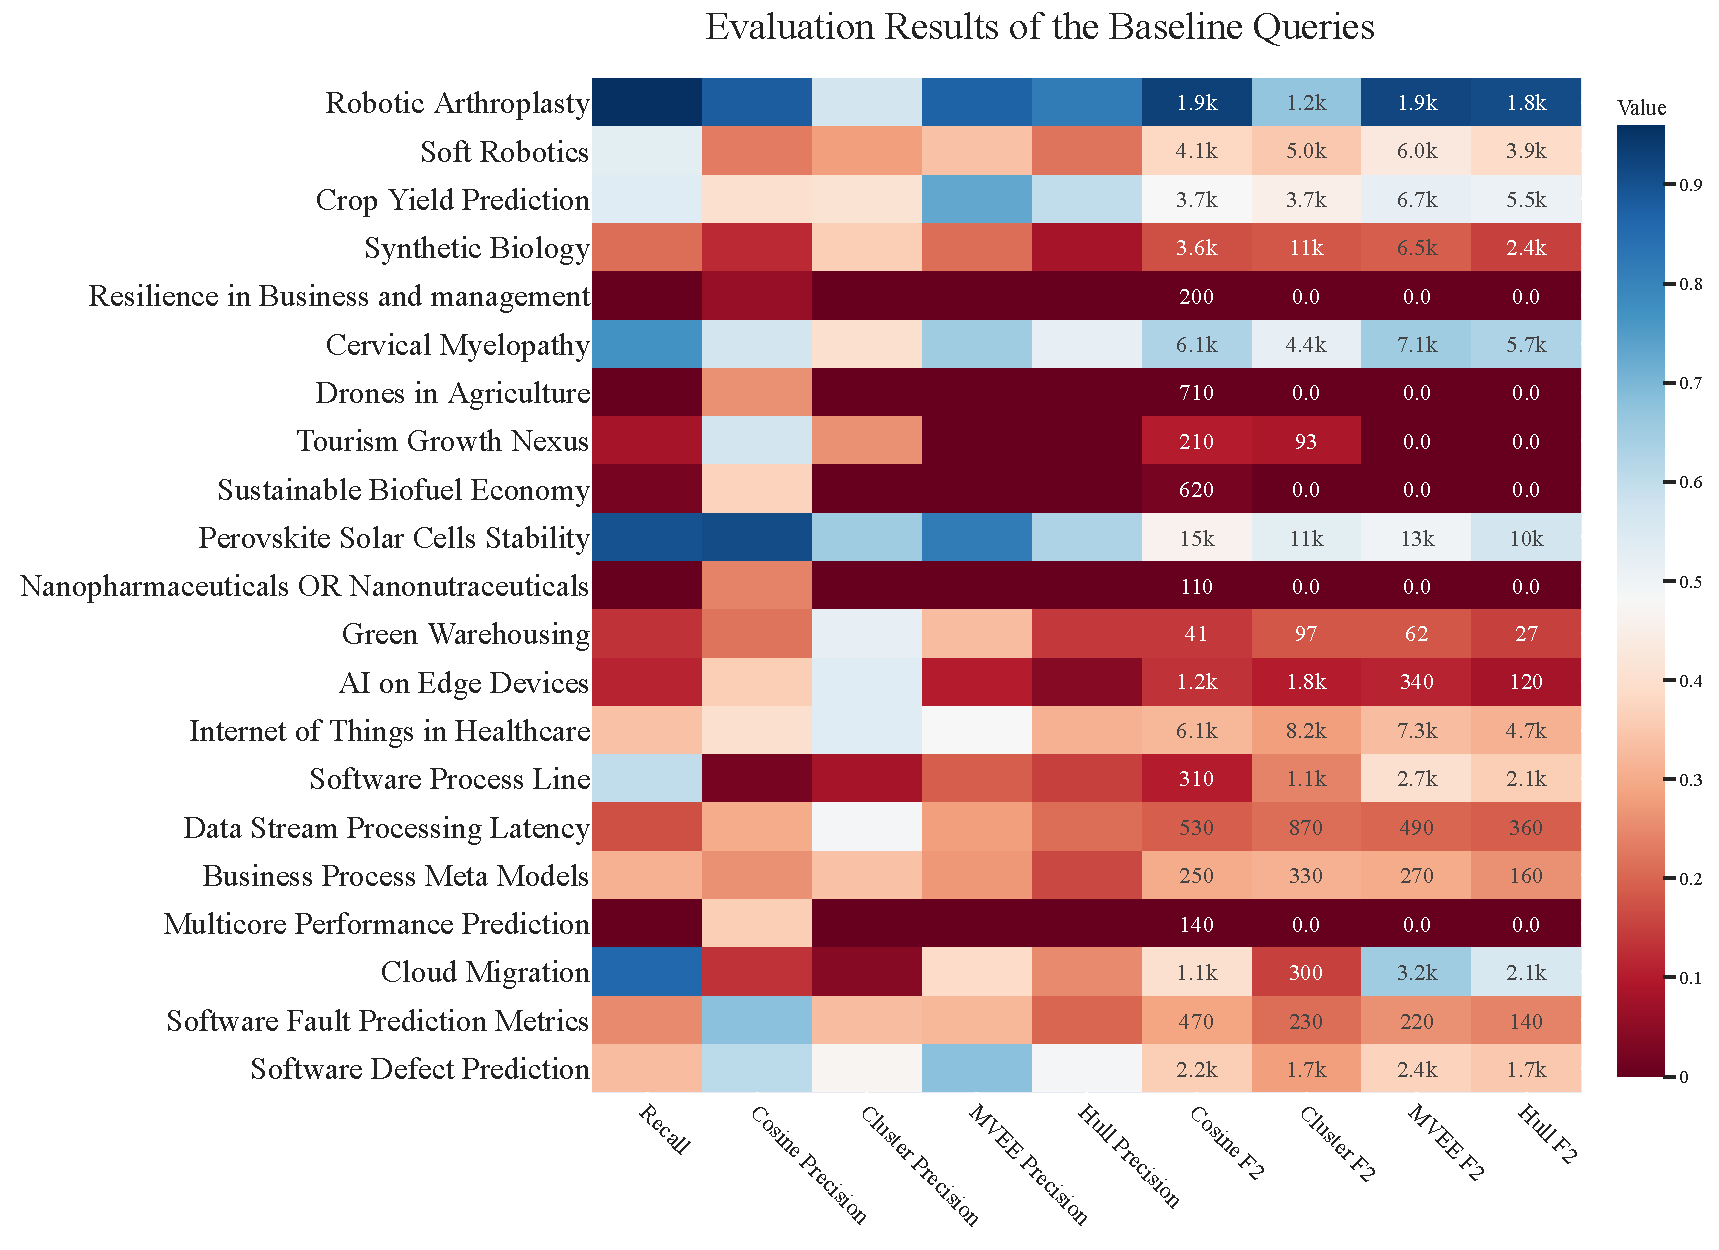
\includegraphics[scale=0.6]{pics/baseline_results.pdf}
	\caption{The evaluation results of the baseline queries. The color in the figure represents the value of the metric in their respective columns, where the text on F2 metrics indicates the total number of relevant publications used to compute the decay factor. The query for \textit{Robotic Arthroplasty} demonstrates strong performance across precision and recall, and containing only 1.9k relevant publications, thus the high F2 score. In contrast, while \textit{Perovskite Solar Cells Stability} achieves high recall and precision, its F2 score is only decent due to the large number of publications. For the rest of the topics, the F2 score is below average mostly due to the low recall.}\label{fig:baseline-results}
	\label{fig:baseline-results}
\end{figure}

\begin{figure}
	\hspace*{-4cm}	
	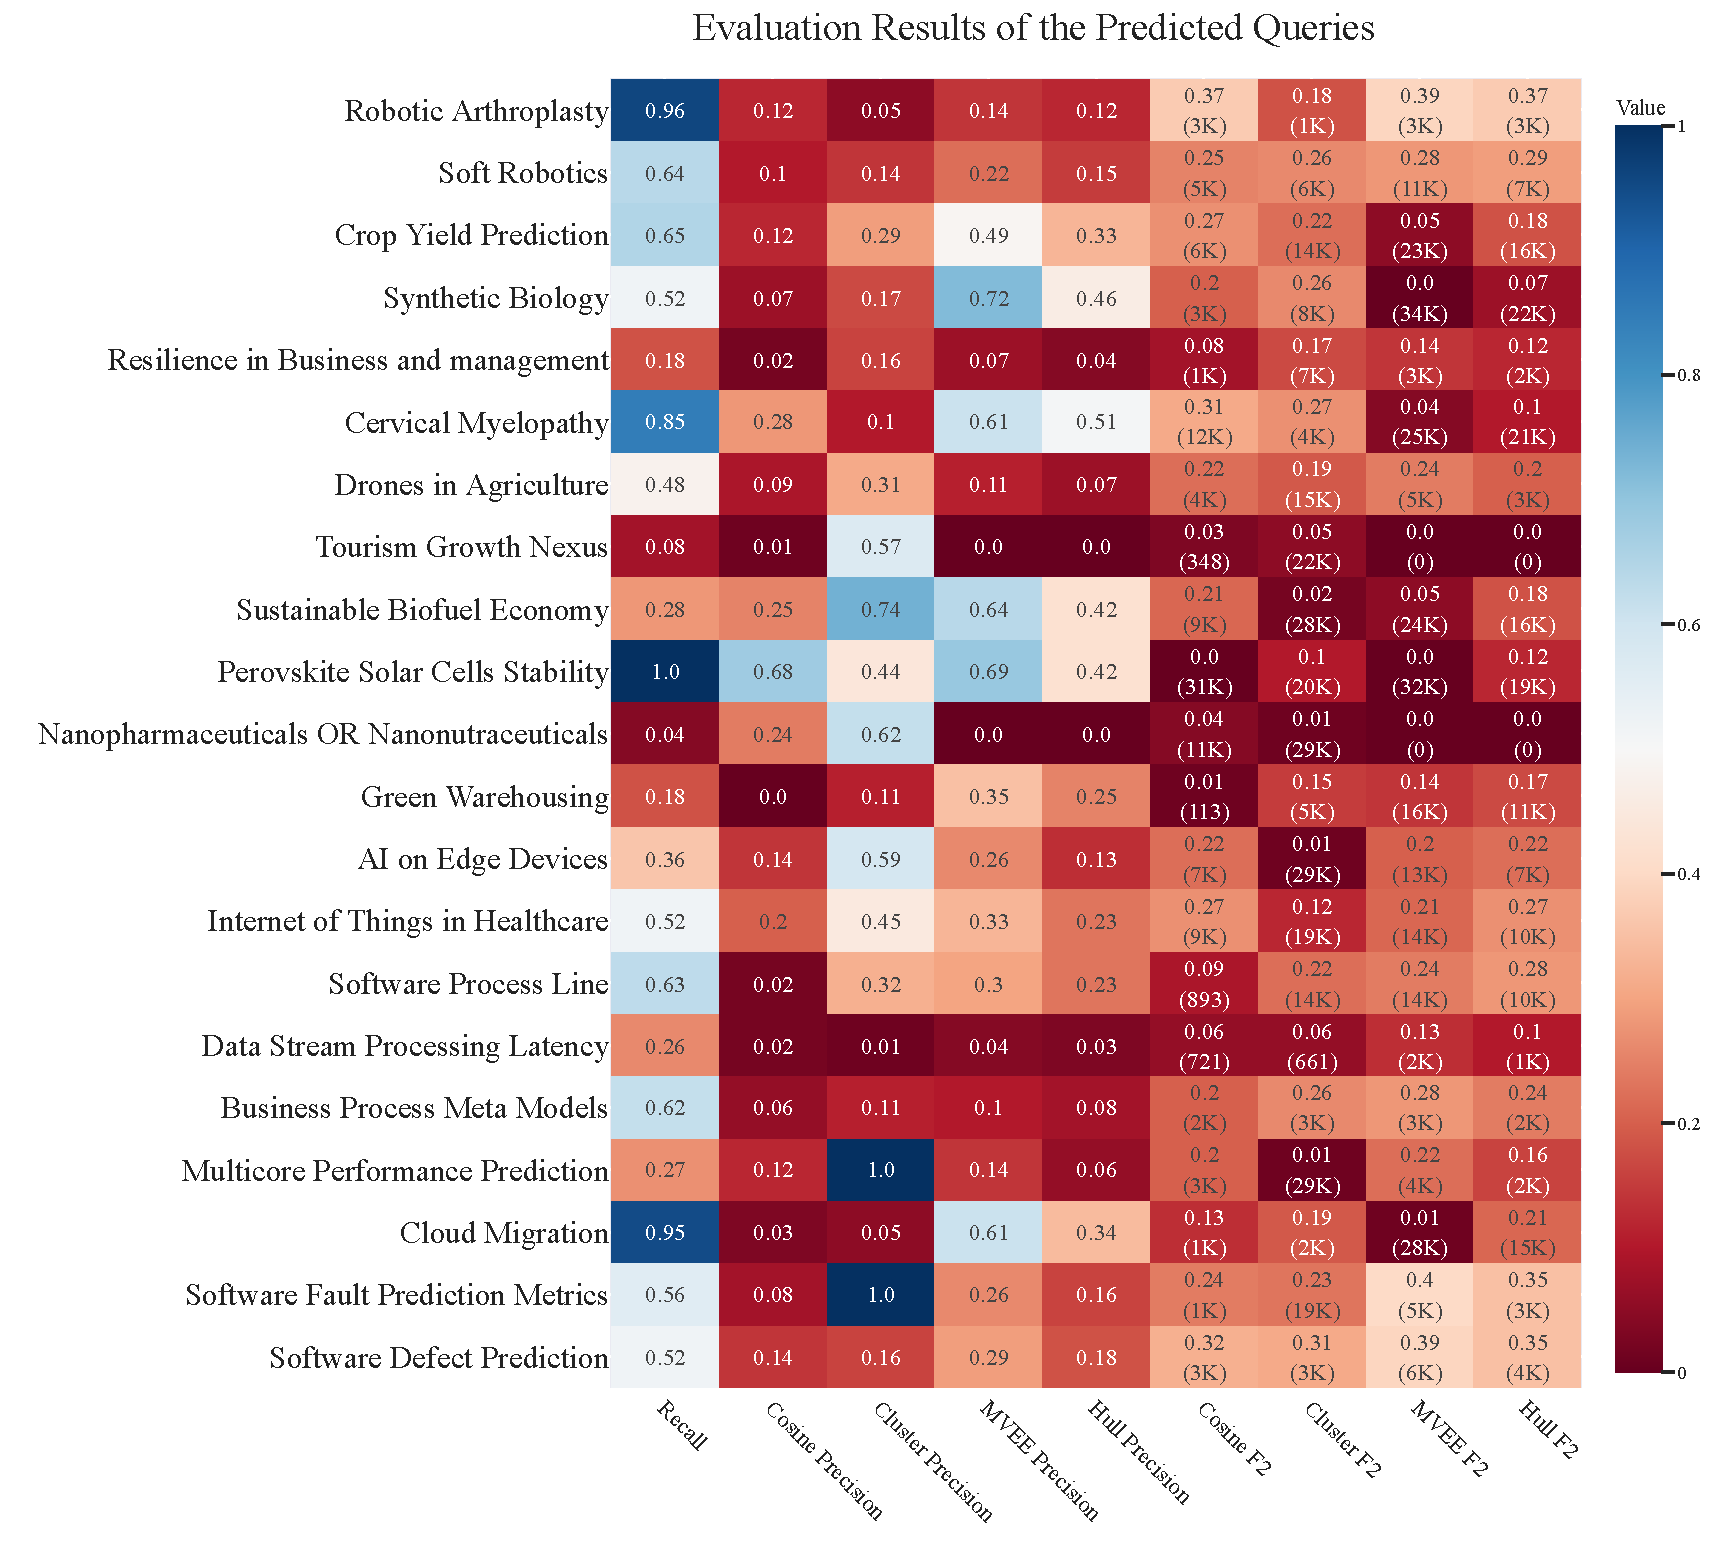
\includegraphics[scale=0.6]{pics/predicted_results.pdf}
	\caption{The evaluation results of the SLR queries. The color in the figure represents the value of the metric in their respective columns, where the text on F2 metrics indicates the total number of relevant publications used to compute the decay factor. The query for \textit{Robotic Arthroplasty} demonstrates strong performance across precision and recall, and containing only 1.9k relevant publications, thus the high F2 score. In contrast, while \textit{Perovskite Solar Cells Stability} achieves high recall and precision, its F2 score is only decent due to the large number of publications. For the rest of the topics, the F2 score is below average mostly due to the low recall.}\label{fig:predicted-results}
\end{figure}

\begin{figure}
	\hspace*{-3cm}	
	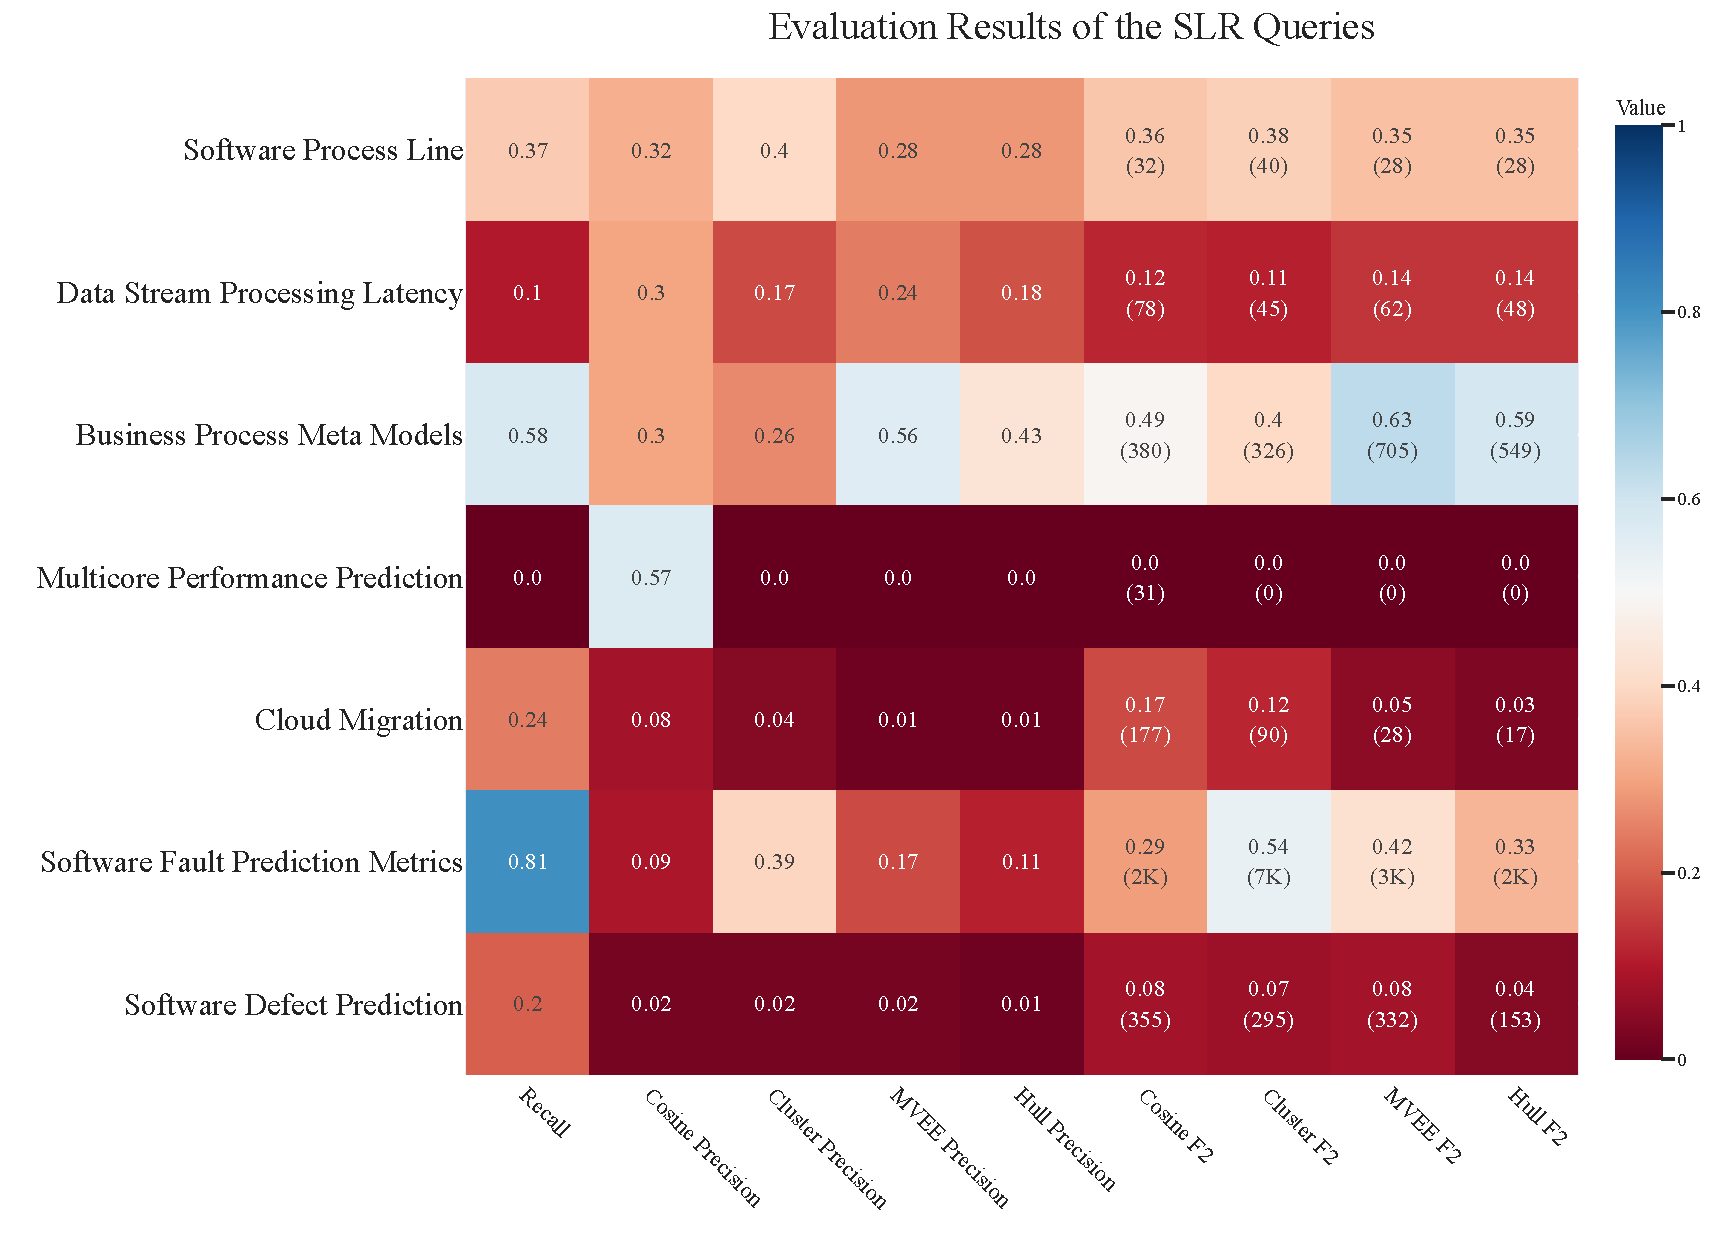
\includegraphics[scale=0.6]{pics/slr_results.pdf}
	\caption{The evaluation results of the SLR queries. The color in the figure represents the value of the metric in their respective columns, where the text on F2 metrics indicates the total number of relevant publications used to compute the decay factor. Overall, the sample size of the handcrafted SLR queries is smaller compared to the baseline and predicted queries. This reduced count facilitates manual screening of results; however, it appears that precision is generally average to low across these queries. Notably, the SLR query used for \textit{Multicore Performance Prediction} is only partially available for public access \autocite{Frank2017}, hence the very low scores.} \label{fig:slr-results}

\end{figure}

\printbibliography

\begingroup
\addcontentsline{toc}{chapter}{\IfLanguageName{ngerman}{Erklärung}{Declaration}}
\chapter*{\IfLanguageName{ngerman}{Erklärung}{Declaration}}
% \thispagestyle{empty}
\IfLanguageName{ngerman}{
Ich versichere, die von mir vorgelegte Arbeit selbstständig verfasst zu haben.
Alle Stellen, die wörtlich oder sinngemäß aus veröffentlichten oder nicht veröffentlichten Arbeiten Dritter entnommen sind, habe ich als solche kenntlich gemacht.
Sämtliche Quellen und Hilfsmittel, die ich für die Arbeit benutzt habe, sind angegeben.

% adapt if tools were used
% remove if no tools have been used
(Es folgen Formulierungsbeispiele, die Sie im Sinne der Transparenz an Ihre Arbeit anpassen müssen. Über die Zulässigkeit von Hilfsmitteln sollten Sie natürlich im Vorfeld mit Ihrem Betreuer diskutiert haben.)
Insb. wurden zur Erstellung dieser Arbeit auch folgende KI Systeme eingesetzt:
\begin{itemize}
    \item ChatGPT in Version ... wurde zur initialen Ausformulierung basierend auf von mir vorgegebenen Stichpunkten in den Kapiteln ... / der gesamten Arbeit eingesetzt.
    \item ChatGPT wurde zu folgenden Themen befragt: ... / zur Generierung von Ideen bzgl. ... / Strukturierung von ... genutzt / zur Konzeption des Systems ... genutzt.
    
    Der Wortlaut der Dialoge, sowie die verwendete Version wurde im Anhang der Arbeit dokumentiert. Genutzte Passagen sind im Text als solche gekennzeichnet.
    \item ChatGPT wurde zur Erstellung von Quellcode für ... genutzt.
    
    Der Wortlaut der Dialoge, sowie die verwendete Version wurde im Anhang der Arbeit dokumentiert. Die Verwendung ist im Kopf der jeweiligen Quelldatei / Klasse / Methode / Teile kenntlich gemacht.
    \item Copilot in Version ... wurde zur Erstellung von Quellcode / Auto-Complete für ... genutzt. Die Verwendung ist im Kopf der jeweiligen Quelldatei / Klasse / Methode / Teile kenntlich gemacht.
\end{itemize}
Mir ist bewusst, dass von KI Systemen generierte Inhalte das sorgfältige wissenschaftliche Arbeiten nicht ersetzen, weshalb sämtliche derartige Inhalte durch mich kritisch überprüft und finalisiert wurden.

Die Arbeit war mit gleichem Inhalt bzw. in wesentlichen Teilen noch nicht Gegenstand einer anderen Prüfung.
}{
I declare that I have written this work by myself.
I have identified as such all passages taken verbatim or in meaning from published or unpublished works by third parties.
All sources and aids that I have used for the work are indicated.

% adapt if tools were used
% remove if no tools have been used
(Example formulations follow, which you must adapt to your work for the sake of transparency. Of course, you should have discussed about the acceptability of such aids with your supervisor in advance.)
In particular, the following AI systems were also used to create this work:
\begin{itemize}
    \item ChatGPT in version ... was used for the initial text drafting based on bullet points given by me in the chapters ... / of the entire work.
    \item ChatGPT was consulted on the following topics: ... / was used to generate ideas regarding ... / for the structuring of ... / for the conception of the system ... .
    
    The wording of the dialogs and the version used were documented in the appendix of this work. Passages used are marked as such in the text.
    \item ChatGPT was used to create source code for ... . The wording of the dialogs and the version used were documented in the appendix of this work. The use is indicated in the header of the respective source file / class / method / parts.
    \item Copilot in version ... was used to create source code / auto-complete for ... . The use is documented in the header of the respective source file / class / method / parts.
\end{itemize}
I am aware that content generated by AI systems is no substitute for careful scientific work, which is why all such generated content has been critically reviewed and finalized by me.

This work has neither been submitted with the same content nor in essential parts to any other examination authority.
}

\bigskip\bigskip
\noindent\textit{\myLocation, \myThesisSubDate}

\smallskip

\begin{flushright}
    \begin{tabular}{m{6cm}}
        \\ \hline
        \centering\myName \\
    \end{tabular}
\end{flushright}

\endgroup






\end{document}
